%% History:
%% May 2019 Tomi Männistö, Antti-Pekka Tuovinen proofreading; 30 vs. 40 cr theses, etc.
%% May 2019 Tomi Männistö changed from babelbib to bibtex; Abstract page (and other pages as well) reformatting.
%% January–May 2019 several issues fixed by Niko Mäkitalo; long fields in abstract
%% March 2018 template file extended by Lea Kutvonen to exploit HYthesisML.cls.
%% Feb2018 This template file for the use of HYgraduML.cls was  modified by Veli Mäkinen from HY_fysiikka_LuKtemplate.tex
%% authored by Roope Halonen ja Tomi Vainio in 2017.
%% Some text is also inherited from engl_malli.tex versions by Kutvonen, Erkiö, Mäkelä, Verkamo, Kurhila, and
%% Nykänen, to accompany tktltiki.cls (by Puolakka 2002).


%% Follow comments to support use.

%%%%%%%%%%%%%%%%%%%%%%%%%%%%%%%%%%%%%%%%%%%%%%%%%%%%%%%%%
%% STEP 1: Choose options for MSc / BSc layout and your bibliographic style
%%%%%%%%%%%%%%%%%%%%%%%%%%%%%%%%%%%%%%%%%%%%%%%%%%%%%%%%%

%%  Language: 
%%      finnish, swedish, or english
%%  Pagination (use twoside by default)  
%%      oneside or twoside,
%%  Study programme / kind of report
%%      csm  = pro gradu in new Computer science MSc;
%%      cs = pro gradu in old Computer Science MSc;
%%      tkt = BSc thesis in new curricula;
%%      tktl= BSc thesis in old curricula;
%%  For MSc choose your line or track:
%%      (30 cr thesis, 2020 onwards, Master of Computer Science programme = csm)
%%      software-track-2020 = Software study track
%%      algorithms-track-2020 = Algorithms study track
%%      networking-track-2020 = Networking study track
%%
%%      (30 cr thesis, Master of Computer Science programme = csm)
%%      sw-track-2018 = Software Systems study track
%%      alko-track-2018 = Algorithms study track
%%      nodes-track-2018 = Networking and Services study track
%%
%%      (30 cr thesis, Master of Computer Science programme = csm)
%%      sw-line-2017 =  Software systems subprogramme
%%      alko-line-2017 = Algorithms, Data Analytics and Machine Learning subprogramme
%%      bio-line-2017 = Algorithmic Bioinformatics subprogramme
%%      nodes-line-2017 = Networking and Services subprogramme
%%
%%      (40 cr thesis, = cs)
%%      sw-line = Software Systems specialisation line 
%%      alko-line = Algorithms specialisation line
%%      bio-line = Algorithmic bioinformatics specialisation line
%%      nodes-line = Networking and Services specialisation line

\documentclass[english,twoside,censored,cs,nodes-line]{HYthesisML}


% In theses, open new chapters only at right page.
% For other types of documents, may ask "openany" in document.
\PassOptionsToClass{openright,twoside,a4paper}{report}
%\PassOptionsToClass{openany,twoside,a4paper}{report}

\usepackage{csquotes}
%%%%%%%%%%%%%%%%%%%%%%%%%%%%%%%%%%%%%%%%%%%%%%%%%%%%%%%%%
%% REFERENCES
%% Some notes on bibliography usage and options:
%% natbib -> you can use, e.g., \citep{} or \parencite{} for (Einstein, 1905); with APA \cite -> Einstein, 1905 without ()
%% maxcitenames=2 -> only 2 author names in text citations, if more -> et al. is used
%% maxbibnames=99 as no great need to suppress the biliography list in a thesis
%% for more information see biblatex package documentation, e.g., from https://ctan.org/pkg/biblatex 

%% Reference style: select one 
%% for APA = Harvard style = authoryear -> (Einstein, 1905) use:
%\usepackage[style=authoryear,bibstyle=authoryear,backend=biber,natbib=true,maxnames=99,maxcitenames=2,giveninits=true,uniquename=init]{biblatex}
%% for numeric = Vancouver style -> [1] use:
\usepackage[style=numeric,bibstyle=numeric,backend=biber,natbib=true,maxbibnames=99,giveninits=true,uniquename=init]{biblatex}
%% for alpahbetic -> [Ein05] use:
%\usepackage[style=alphabetic,bibstyle=alphabetic,backend=biber,natbib=true,maxbibnames=99,giveninits=true,uniquename=init]{biblatex}
%

\addbibresource{bibliography.bib}
% in case you want the final delimiter between authors & -> (Einstein & Zweistein, 1905) 
% \renewcommand{\finalnamedelim}{ \& }
% List the authors in the Bibilipgraphy as Lastname F, Familyname G,
\DeclareNameAlias{sortname}{family-given}
% remove the punctuation between author names in Bibliography 
%\renewcommand{\revsdnamepunct}{ }


%% Block of definitions for fonts and packages for picture management.
%% In some systems, the figure packages may not be happy together.
%% Choose the ones you need.

%\usepackage[utf8]{inputenc} % For UTF8 support, in some systems. Use UTF8 when saving your file.

\usepackage{lmodern}         % Font package, again in some systems.
\usepackage{textcomp}        % Package for special symbols
\usepackage[pdftex]{color, graphicx} % For pdf output and jpg/png graphics
\usepackage{epsfig}
\usepackage{subfigure}
\usepackage[pdftex, plainpages=false]{hyperref} % For hyperlinks and pdf metadata
\usepackage{fancyhdr}        % For nicer page headers
\usepackage{tikz}            % For making vector graphics (hard to learn but powerful)
%\usepackage{wrapfig}        % For nice text-wrapping figures (use at own discretion)
\usepackage{amsmath, amssymb} % For better math

\usepackage{latexsym}

\usepackage{algpseudocode}

\usepackage{pgf-pie}
\usepackage{pgfplots}

\pgfplotsset{width=9cm,compat=1.8}

\usetikzlibrary{backgrounds,calc,shadings,shapes.arrows,shapes.symbols,shadows}
\definecolor{switch}{HTML}{006996}

\makeatletter
\pgfkeys{/pgf/.cd,
  parallelepiped offset x/.initial=2mm,
  parallelepiped offset y/.initial=2mm
}
\pgfdeclareshape{parallelepiped}
{
  \inheritsavedanchors[from=rectangle] % this is nearly a rectangle
  \inheritanchorborder[from=rectangle]
  \inheritanchor[from=rectangle]{north}
  \inheritanchor[from=rectangle]{north west}
  \inheritanchor[from=rectangle]{north east}
  \inheritanchor[from=rectangle]{center}
  \inheritanchor[from=rectangle]{west}
  \inheritanchor[from=rectangle]{east}
  \inheritanchor[from=rectangle]{mid}
  \inheritanchor[from=rectangle]{mid west}
  \inheritanchor[from=rectangle]{mid east}
  \inheritanchor[from=rectangle]{base}
  \inheritanchor[from=rectangle]{base west}
  \inheritanchor[from=rectangle]{base east}
  \inheritanchor[from=rectangle]{south}
  \inheritanchor[from=rectangle]{south west}
  \inheritanchor[from=rectangle]{south east}
  \backgroundpath{
    % store lower right in xa/ya and upper right in xb/yb
    \southwest \pgf@xa=\pgf@x \pgf@ya=\pgf@y
    \northeast \pgf@xb=\pgf@x \pgf@yb=\pgf@y
    \pgfmathsetlength\pgfutil@tempdima{\pgfkeysvalueof{/pgf/parallelepiped
      offset x}}
    \pgfmathsetlength\pgfutil@tempdimb{\pgfkeysvalueof{/pgf/parallelepiped
      offset y}}
    \def\ppd@offset{\pgfpoint{\pgfutil@tempdima}{\pgfutil@tempdimb}}
    \pgfpathmoveto{\pgfqpoint{\pgf@xa}{\pgf@ya}}
    \pgfpathlineto{\pgfqpoint{\pgf@xb}{\pgf@ya}}
    \pgfpathlineto{\pgfqpoint{\pgf@xb}{\pgf@yb}}
    \pgfpathlineto{\pgfqpoint{\pgf@xa}{\pgf@yb}}
    \pgfpathclose
    \pgfpathmoveto{\pgfqpoint{\pgf@xb}{\pgf@ya}}
    \pgfpathlineto{\pgfpointadd{\pgfpoint{\pgf@xb}{\pgf@ya}}{\ppd@offset}}
    \pgfpathlineto{\pgfpointadd{\pgfpoint{\pgf@xb}{\pgf@yb}}{\ppd@offset}}
    \pgfpathlineto{\pgfpointadd{\pgfpoint{\pgf@xa}{\pgf@yb}}{\ppd@offset}}
    \pgfpathlineto{\pgfqpoint{\pgf@xa}{\pgf@yb}}
    \pgfpathmoveto{\pgfqpoint{\pgf@xb}{\pgf@yb}}
    \pgfpathlineto{\pgfpointadd{\pgfpoint{\pgf@xb}{\pgf@yb}}{\ppd@offset}}
  }
}
\makeatother

\tikzset{ports/.style={
    line width=0.3pt,
    top color=gray!20,
    bottom color=gray!80
  },
  rack switch/.style={
    parallelepiped,fill=white, draw,
    minimum width=1.25cm,
    minimum height=0.25cm,
    parallelepiped offset x=2mm,
    parallelepiped offset y=1.25mm,
    xscale=-1,
    path picture={
      \draw[top color=gray!5,bottom color=gray!40]
      (path picture bounding box.south west) rectangle
      (path picture bounding box.north east);
      \coordinate (A-west) at ([xshift=-0.2cm]path picture bounding box.west);
      \coordinate (A-center) at ($(path picture bounding box.center)!0!(path
        picture bounding box.south)$);
      \foreach \x in {0.275,0.525,0.775}{
        \draw[ports]([yshift=-0.05cm]$(A-west)!\x!(A-center)$)
          rectangle +(0.1,0.05);
        \draw[ports]([yshift=-0.125cm]$(A-west)!\x!(A-center)$)
          rectangle +(0.1,0.05);
       }
      \coordinate (A-east) at (path picture bounding box.east);
      \foreach \x in {0.085,0.21,0.335,0.455,0.635,0.755,0.875,1}{
        \draw[ports]([yshift=-0.1125cm]$(A-east)!\x!(A-center)$)
          rectangle +(0.05,0.1);
      }
    }
  },
  server/.style={
    parallelepiped,
    fill=white, draw,
    minimum width=0.35cm,
    minimum height=0.75cm,
    parallelepiped offset x=3mm,
    parallelepiped offset y=2mm,
    xscale=-1,
    path picture={
      \draw[top color=gray!5,bottom color=gray!40]
      (path picture bounding box.south west) rectangle
      (path picture bounding box.north east);
      \coordinate (A-center) at ($(path picture bounding box.center)!0!(path
        picture bounding box.south)$);
      \coordinate (A-west) at ([xshift=-0.575cm]path picture bounding box.west);
      \draw[ports]([yshift=0.1cm]$(A-west)!0!(A-center)$)
        rectangle +(0.2,0.065);
      \draw[ports]([yshift=0.01cm]$(A-west)!0.085!(A-center)$)
        rectangle +(0.15,0.05);
      \fill[black]([yshift=-0.35cm]$(A-west)!-0.1!(A-center)$)
        rectangle +(0.235,0.0175);
      \fill[black]([yshift=-0.385cm]$(A-west)!-0.1!(A-center)$)
        rectangle +(0.235,0.0175);
      \fill[black]([yshift=-0.42cm]$(A-west)!-0.1!(A-center)$)
        rectangle +(0.235,0.0175);
    }
  },
}

\usetikzlibrary{calc, shadings, shadows, shapes.arrows}

% Styles for interfaces and edge labels
\tikzset{%
  interface/.style={draw, rectangle, rounded corners, font=\LARGE\sffamily},
  ethernet/.style={interface, fill=yellow!50},% ethernet interface
  serial/.style={interface, fill=green!70},% serial interface
  speed/.style={sloped, anchor=south, font=\large\sffamily},% line speed at edge
  route/.style={draw, shape=single arrow, single arrow head extend=4mm,
    minimum height=1.7cm, minimum width=3mm, white, fill=switch!20,
    drop shadow={opacity=.8, fill=switch}, font=\tiny}% inroute/outroute arrows
}
\newcommand*{\shift}{1.3cm}% For placing the arrows later

% The router icon
\newcommand*{\router}[1]{
\begin{tikzpicture}
  \coordinate (ll) at (-3,0.5);
  \coordinate (lr) at (3,0.5);
  \coordinate (ul) at (-3,2);
  \coordinate (ur) at (3,2);
  \shade [shading angle=90, left color=switch, right color=white] (ll)
    arc (-180:-60:3cm and .75cm) -- +(0,1.5) arc (-60:-180:3cm and .75cm)
    -- cycle;
  \shade [shading angle=270, right color=switch, left color=white!50] (lr)
    arc (0:-60:3cm and .75cm) -- +(0,1.5) arc (-60:0:3cm and .75cm) -- cycle;
  \draw [thick] (ll) arc (-180:0:3cm and .75cm)
    -- (ur) arc (0:-180:3cm and .75cm) -- cycle;
  \draw [thick, shade, upper left=switch, lower left=switch,
    upper right=switch, lower right=white] (ul)
    arc (-180:180:3cm and .75cm);
  \node at (0,0.5){\color{blue!60!black}\Huge #1};% The name of the router
  % The four arrows, symbols for incoming and outgoing routes:
  \begin{scope}[yshift=2cm, yscale=0.28, transform shape]
    \node[route, rotate=45, xshift=\shift] {\strut};
    \node[route, rotate=-45, xshift=-\shift] {\strut};
    \node[route, rotate=-135, xshift=\shift] {\strut};
    \node[route, rotate=135, xshift=-\shift] {\strut};
  \end{scope}
\end{tikzpicture}}

\makeatletter
\pgfdeclareradialshading[tikz@ball]{cloud}{\pgfpoint{-0.275cm}{0.4cm}}{%
  color(0cm)=(tikz@ball!75!white);
  color(0.1cm)=(tikz@ball!85!white);
  color(0.2cm)=(tikz@ball!95!white);
  color(0.7cm)=(tikz@ball!89!black);
  color(1cm)=(tikz@ball!75!black)
}
\tikzoption{cloud color}{\pgfutil@colorlet{tikz@ball}{#1}%
  \def\tikz@shading{cloud}\tikz@addmode{\tikz@mode@shadetrue}}
\makeatother

\tikzset{my cloud/.style={
     cloud, draw, aspect=2,
     cloud color={gray!5!white}
  }
}


\singlespacing               %line spacing options; normally use single

\fussy
%\sloppy                      % sloppy and fussy commands can be used to avoid overlong text lines
% if you want to see which lines are too long or have too little stuff, comment out the following lines
% \overfullrule=1mm
% to see more info in the detailed log about under/overfull boxes...
% \showboxbreadth=50 
% \showboxdepth=50



%%%%%%%%%%%%%%%%%%%%%%%%%%%%%%%%%%%%%%%%%%%%%%%%%%%%%%%%%
%% STEP 2:
%%%%%%%%%%%%%%%%%%%%%%%%%%%%%%%%%%%%%%%%%%%%%%%%%%%%%%%%%
%% Set up personal information for the title page and the abstract form.
%% Replace parameters with your information.
\title{Automated Software Configuration for Cloud Deployment}

% TM: Contributors to template editors now listed in the beginning of the file in comments
\author{Antero Vainio}
\date{\today}



% Set supervisors and examiners, use the titles according to the thesis language
% Prof. 
% Dr. or in Finnish toht. or tri or FT, TkT, Ph.D. or in Swedish... 
\supervisors{Lirim Osmani, Ashwin Rao, Kalle Happonen}
\examiners{Prof. Sasu Tarkoma}


\keywords{Networking, Virtualization, Distributed Systems}
\additionalinformation{Cloud Computing, IaaS, Software Automation, System
Administration, DevOps, IaC}

%% For seminar papers and such, cover page and abstract
%% requires these three basic items of information.
%% Label as needed and remove comment marks.
%%\level{Seminaariraportti}
%%\programme{Tietojenkäsittelytieteen andidaattiohjelma}
%%\subject{Seminaarisarjan nimi}

%% Replace classification terms with the ones that match your work. ACM
%% ACM Digital library provides a taxonomy and a tool for classification
%% in computer science. Use 1-3 paths, and use right arrows between the
%% about three levels in the path; each path requires a new line.

\classification{\protect{\ \\
\  Networks $\rightarrow$ Network services  $\rightarrow$ Cloud computing\  \\
\  Software and its engineering  $\rightarrow$ Software creation and management  $\rightarrow$ Software post-development issues $\rightarrow$ System administration
}}

%% if you want to quote someone special. You can comment this line out and there will be nothing on the document.
%\quoting{Bachelor's degrees make pretty good placemats if you get them laminated.}{Jeph Jacques}


%% OPTIONAL STEP: Set up properties and metadata for the pdf file that pdfLaTeX makes.
%% Your name, work title, and keywords are recommended.
\hypersetup{
    unicode=true,           % to show non-Latin characters in Acrobat’s bookmarks
    pdftoolbar=true,        % show Acrobat’s toolbar?
    pdfmenubar=true,        % show Acrobat’s menu?
    pdffitwindow=false,     % window fit to page when opened
    pdfstartview={FitH},    % fits the width of the page to the window
    pdftitle={},            % title
    pdfauthor={},           % author
    pdfsubject={},          % subject of the document
    pdfcreator={},          % creator of the document
    pdfproducer={pdfLaTeX}, % producer of the document
    pdfkeywords={something} {something else}, % list of keywords for
    pdfnewwindow=true,      % links in new window
    colorlinks=true,        % false: boxed links; true: colored links
    linkcolor=black,        % color of internal links
    citecolor=black,        % color of links to bibliography
    filecolor=magenta,      % color of file links
    urlcolor=cyan           % color of external links
}

%%-----------------------------------------------------------------------------------

\begin{document}

% Generate title page.
\maketitle


%%%%%%%%%%%%%%%%%%%%%%%%%%%%%%%%%%%%%%%%%%%%%%%%%%%%%%%%%
%% STEP 3:
%%%%%%%%%%%%%%%%%%%%%%%%%%%%%%%%%%%%%%%%%%%%%%%%%%%%%%%%%
%% Write your abstract to be positioned here.
%% You can make several abstract pages (if you want it in different languages),
%% but you should also then redefine some of the above parameters in the proper
%% language as well, in between the abstract definitions.

\begin{abstract}

Internet is nowadays being used as a platform for providing a wide variety of
different services. This has created challenges related to scaling IT
infrastructure management. Cloud computing is a popular solution for scaling
infrastructure, either by building a self-hosted cloud or by using cloud
platform provided by external organizations. This transfers some the challenges
related to large scale to the cloud administrators.

OpenStack is a group of open-source software projects for running cloud
platforms. It is the most commonly used software for building private clouds.
Since initially published by NASA and Rackspace, it has been used by various
organizations such as Walmart, China Mobile and Cern nuclear research
institute. Largest production deployments of OpenStack clouds consist of
thousands of physical server computers located in multiple datacenters.

OpenStack community has created many deployment methods that take advantage of
automated software configuration management. Methods are built with state of
the art software for automating different administrative tasks. Deployment
methods take different approaches to automating infrastructure management for
OpenStack.

This paper compares some of the automated deployment methods being used and
reflects on some of the benefits of using automation for configuration
management. Comparisons are based on technical documentation and reference
literature. A questionnaire related to the use of automation was conducted for
OpenStack administrators. Lastly, one of the deployment methods was tested in a
virtualized environment.

\end{abstract}

% Place ToC
\newpage
\mytableofcontents
\mainmatter

%%%%%%%%%%%%%%%%%%%%%%%%%%%%%%%%%%%%%%%%%%%%%%%%%%%%%%%%%
%% STEP 4: Write the thesis.
%%%%%%%%%%%%%%%%%%%%%%%%%%%%%%%%%%%%%%%%%%%%%%%%%%%%%%%%%
%% Your actual text starts here. You shouldn't mess with the code above the line except
%% to change the parameters. Removing the abstract and ToC commands will mess up stuff.
%%
%% You may wish to include material to avoid browsing the definitions
%% above. Command \include{file} includes the file of name file.tex.
%% As a side effect, subsequent inclusions may force a page break.

% BSc instructions
%\include{bsc_finnish_contents}
%\include{bsc_english_contents}
% MSc instructions
%\include{msc_finnish_contents}
\chapter{Introduction}

As providing services over the Internet has become a common practice in the
modern society, maintenance of information systems has encountered many
challenges as well. While web-based applications have become more diverse,
resource-intensive, and complicated, they face higher expectations with respect
to usability, performance and security.

Often times industrial software development has strict deadlines to follow.
Many development practices are built around the idea of constant service
improvement. It means that a software product is rarely considered finished but
instead new features are being added to it and flaws being fixed in a priority
order.

As a result, programs and sometimes entire system architectures tend to require
frequent updates. Similarly to IT services automating repetitive tasks in hopes
of achieving reliability and cost-effectiveness, software development processes
aim to utilize automation whenever feasible.

Cloud enviroments offer on-demand computing resources for cloud consumers. When
deploying to cloud, a user can expect customized servers being provisioned
within seconds. It can be achieved with a combination of hypervisors and
programs preinstalled in virtual machines for instance. For further
configurations, additional software automation tools can be used.

Cloud environments are formed by physical host machines that lease virtualized
devices such as virtual CPUs (vCPU), logical volumes, or virtual network
devices. Users get typically charged for the time that they use some of these
resources. Servers can quickly be set up and down, preventing users from
having to pay for under-utilized servers.

For server provisioning, cloud providers do not typically have the same
luxuries as cloud users, since using virtualization is not optimal due to added
processing overhead. However when it comes to configuring hundreds or even
thousands of physical server computers, automation is once again seen as a
potential solution. Yet many traditional cloud administrators are still relying
on manual maintenance operations.

This thesis explores different popular methods for deploying and administering
cloud environments with help of software automation. Selected automation tools
and de facto methods for using them are compared. Questions \ref{fig:rqs} are
reflected during evaluation.

Deployed software is a combination OpenStack services. OpenStack is a
collective of open-source software projects for running cloud servers.
OpenStack is the most widely used plaftorm for creating private clouds. It
includes official repositories for various automated deployment methods. Most
of the methods provide a basis on which to build a solution customized for own
working environment.

\begin{figure}[t]
\centering
\begin{itemize}
  \item [RQ1] What are the key factors affecting the design of different
              deployment methods, and how do they differentiate from each
              other?
  \item [RQ2] What kind of features do different deployment methods offer?
              Which components are used in deployments?
  \item [RQ3] Who will benefit from the development of software automation
              tools, and why?
\end{itemize}
\caption{Research Questions}
\label{fig:rqs}
\end{figure}

\chapter{State Of The Art}

This thesis is motivated by current trends and contemporary practices used for
administering IT infrastructures. Cloud computing has reached nearly a de facto
status for large scale infrastructure provisioning. While cloud services
automate many administrative tasks, another increasingly utilized method in IT
service management is the use of software automation for system configurations.

Usually whenever there is a trend or a commonly followed practice in the field
of computer science, there are various approaches taken to achieve it.
Different approaches may share similarities in some aspects while at the same
time they can be fundamentally different in other aspects. One of the reasons
for the existence of various alternative solutions can be commercial
competition, another can bedifferent preferences for software architectures.

There is a lot of diversity when it comes to the use of software solutions for
IT service management. However for the most parts IT services themselves have
similar requirements related to the quality of service. Services have
requirements such as highly availability, reliability, efficiency, usability,
and security. At the same time service management needs to be cost-efficient.
When it comes to providing high quality with low cost, proper use of automated
solutions may prove to be valuable.

With successful Internet based services, scale makes a big difference. Spikes
in the number of active users can affect the quality of service significantly,
even to the point where the service is unusable. At the same time, having
under-utilized servers wastes resources and thus increases the cost of
providing service, resulting in competitive disadvantage in the market. This
must be considered both in the design of the application software and in the
infrastructure architecture.

Number of users for a web-based application can change a lot during the course
of a regular business day. Many services have repeating patterns in their
level of usage and the number of users for a particular time of day can be
predicted with high accuracy. If usage level has drastic changes and follows a
repeating pattern, provisioned computing resources can be scaled correspondinly
resulting in cost savings for optimized resource utilization. With the help of
detailed analysis and the use of cloud platforms, this can be achieved.

When scaling infrastructure, many administrative tasks become repetitive. When
scaling up, deployed applications need to be configured and integrated to
environment. When scaling down, it has to be ensured that no application is
requesting removed application instances. When done manually these tasks have a
high risk of failure due to human error to the point where they cannot be
expected to be frequently without this adding a lot of costs.

Even when infrastructure is not scaled rapidly, there are repeating
administrative tasks, such as software updates and hardware maintentance
operations. Having to assure service operations during maintenance suffers the
same risk of human error, when relying on manual operations. Still this is a
practice for many administrators and may even limit the potential of the
provided IT service.

Cloud computing can be used for provisioning computing resources rapidly. For
customized applications, additional configuration is often necessary. Software
configuration management is a potential solution for avoiding human error in
repetitive configuration tasks as it enables these configurations to be applied
programmatically. While providing operational reliability, it has additional
benefits such as fast execution, and documentation value provided formally
defined configuration tasks.

Another recent trend in IT service management is the DevOps movement. The term
DevOps is often used to describe a principle of speeding up development by
simplifying the process of publishing new software versions. By using efficient
development processes and automated tools, the time it takes to
deploy a new software version to runtime environment or package distribution
can be cut, lowering the overall cost of IT development. DevOps movement was
motivated by agile software development principles and the realization that
communication between software developers and operators often times ended up
being an unnecessary bottleneck for project speed.

Some of the goals of DevOps movement, such as fast and automated software
release process, can be achieved with a proper use of cloud platforms and
software configuration management tools. They allow application developers to
define the deployment process either completely or partially. Deployment is
executed by running applications as opposed to manually following with
application specific instructions. Use of automation avoids errors resulting
from miscommunication between developers and operators.

This chapter provides a short introduction to the concepts behind cloud
computing and software confuration management. Some contemporary software
solutions for these concepts. Descriptions aim to provide answers to research
question RQ1 shown on Figure \ref{fig:rqs}. Key design principles and
differences of the tools are presented as they will affect any deployment
methods related to them.

\section{Cloud Computing}

For the last decade, cloud computing has been a common paradigm for IT
infrastructure management. It provides benefits such as high server utilization
and dynamic scalability with a pay-as-you-go price model for outsourced server
infrastructure. Cloud computing is being widely used in various industrial
fields, including telecommunication, retail, finance, and scientific research.
As a result, there is also an inreasing number of public cloud platforms
available, most notably Amazon Web Services (AWS) \citep{aws}, Microsoft Azure
\cite{azure}, and Google Cloud Platform (GCP) \cite{gcp}.

As with many practices in the field of computer science, cloud computing lacks
a universally agreed formal definition. However common to most of the
contemporary cloud platforms is the ability for the end user to provision
computing resources over HTTP interfaces, mostly by using Restful APIs. This
makes it possible to automate infrastructure provisioning. Cloud consumer
avoids the need to request infrastructure operations from administrators, while
administrators don't have to spend time for repetitive tasks related to
infrastructure provisioning.

Due to its on-demand nature, a term often used to describe cloud resource
provisioning model is \textit{Infrastructure-as-a-Service} (IaaS). It
emphasizes the fact that infrastructure can be provisioned through a
well-defined interface. IaaS can be generalized to term
\textit{Anything-as-a-Service} (XaaS), where anything stands for any resource
that is provided through programmable interfaces. Whereas in IaaS, the provided
resources are relatively low-level computing resources, such as servers,
networks or volumes, in \textit{Software-as-a-Service} model, in addition to
service provider provisioning infrastructure, it takes care of software
licencing and configuration.

Reason for varying service models offered by cloud providers, is the fact that
clients have varying needs in terms of outsourced software solutions. Some
clients may want an easily adaptable software configuration with no need for
additional configurations and expertice related to the software; in case of
issues with the software they are willing to pay for customer support. At the
same time there are clients who use cloud providers only for leasing
infrastructure in order to avoid having to maintain own data centers. For the
first type of client, SaaS may be the right service model, and the latter might
prefer IaaS.

When it comes to providing XaaS model services, cloud service providers have
advantages for making new products. As they know their cloud platform in
detail, they are able to produce optimized solutions for particular use cases.
They also have full access to their platform, making it possible to avoid any
workaround solutions that may arise from having to tailor solutions to
interfaces provided by other services.

Reasons why some clients may still prefer to configure software being hosted on
cloud platforms themselves, are saves in costs, and the ability to tailor
solutions to their particular needs. XaaS products have to be generalized
enough so that they can be used by a large customer base. The more a product is
generalized, the less it can be directly adapted to a particular use case.
There are different approaches to dealing with this dilemma, such as
configuration options or large catalogs of tailored services.

Another characteristic in cloud environments is seemingly limitless resources
available on-demand, enabling the infrastructure to be scaled rapidly based on
current usage. As cloud platforms can be used for various computational tasks,
investing in large data centers is more reliable for cloud providers than for
any particular industrial field practicioner.

With more computing resources available, and the ability to provision them for
an execution of a particular computational task with no extra cost, some cloud
consumers may use the platform to lease many vCPU hours for a short period of
time, instead of using less vCPU hours for a longer period of time. This way of
using cloud platform is more typical with computational applications such as
with business analytics, and scientific research.

Ability to think of a cloud platform as having limitless computing resources
makes it possible to consider cloud platforms alternatives for \textit{High
Performance Computing} (HPC) or \textit{High Throughput Computing} (HTC). In
general this would be achieved by scaling computations horizontally. If a heavy
computational task can be split to subtasks that can be run in parallel, they
can be executed on different hardware, shortening the overall time of
computation. Similarly, if a large data stream can be split to smaller streams
to be combined at receiver, the overall time of transmission can be shortened
by using different network links. MapReduce \cite{mapreduce} is an application
developed to help parallelize computational tasks by defining them as map and
reduce fuctions. This model makes it possible to parallelize and thus scale
computations horizontally by the runtime system.

Although cloud platforms primarily provide scalability horizontally with a
number of provisioned instances, some of the larger cloud platforms provide
also instance flavors with highly performant computing hardware. These flavors
may be provided for bare metal services to reduce computational overhead of
virtualization. While vertical scaling is not a feature distinct to cloud
platforms, they benefit from the high user base. This way while the platform
grows, as more varying computing flavors are being provided, computers with
high-quality CPUs and GPUs can be aquired in hopes that they will not go
unutilized.

Cloud environments may be public or private. While public and private cloud
services do not functionally differ from one another, private cloud services
are restricted to particular end users and public cloud services are offered
more or less without restrictions. As a result, generally public cloud
environments are larger in size, known examples of such environments include
AWS, Azure and GCP.

Some cloud platforms are built on top of a number of other cloud platforms.
Such architectures are called \textit{multi clouds}. Multi clouds may use a
particular cloud provider for certain types of resources, such as virtual
networks to be able to use quality wide area network infrastructure. They may
also use other cloud platforms for provisioning resources that they do not have
available at the moment.

\subsection{OpenStack}

OpenStack \cite{openstack} is the most widely used open-source software for
building cloud environments. It was originally developed by NASA and Rackspace,
and published openly in the year 2010. Since then it has been developed by
various organizations, including Cern nuclear research institute as well as
individual contributors. It has been battle-proven for a reliable cloud
operation \cite{forrester}. While OpenStack can be used for public clouds, it
is most commonly used for private clouds or multi clouds. It is currently being
also developed to provide support for edge computing infrastructures.

At its core OpenStack is an example of a IaaS platform. It provides
functionality for infrastructure provisioning through various services.
Infrastructure provisioning is also the primary use case of OpenStack for most
of its users. Many of the OpenStack services can be extended for providing
XaaS, such as VPN-as-a-Service or Database-as-a-Service. Some of these
extensions can be installed as plugins for the appropriate OpenStack services.
Otherwise any extensions have to be implemented.

In addition to installing OpenStack with low-level open-source projects,
OpenStack community has an official marketplace for commercial high-level
OpenStack-based software products. Commercial OpenStack products may provide
official integration to other platforms, or simplify and provide support for
the installation of OpenStack.

OpenStack consists of different services, not all of which are required for an
operational cloud. OpenStack services may also be used as a part of other
distributed systems without deploying a full OpenStack cloud. At basic level,
OpenStack services are Python application servers and related worker agents.
They use other infrastructure services, such as message queues, databases,
caches and proxies.

In order to grant access to resources, OpenStack services need to be able to
authenticate and authorize requestors, which may be end users or other
services. Amongst OpenStack services, Keystone provides Identity and Access
Management in cloud. Since OpenStack services use it for access control when
communicating with other services it is the first service to be installed in
an OpenStack deployment.

An essential resource in any computing environment is the actual computing
units. Traditionally OpenStack has provided computing resources by using
hypervisors, such as ESXI or KVM/QEMU. OpenStack compute service is called
Nova and it was one of the first services developed. Nova receives requests
that describe the specifications for needed virtual machines. Nova then
schedules the creation of the virtual machine from the hypervisor.

In order to access virtual machines created by Nova, network access is
required. Virtual network devices are used for on-demand network provisioning.
Originally virtual networks were provided by Nova service, but currenlty there
is a specific OpenStack service, called Neutron, that is responsible for
network provisioning. Even though nova-network is considered legacy, older
OpenStack deployments are still using it as they have not been updated to
support Neutron. As an example, Cern which has been a long-time OpenStack user,
is still using nova-network in its deployment.

Virtual machine images used by Nova are provided by Glance. Typically guest
operating system images are built by cloud administrator by using tools such as
disk-image-builder. However users are able to create virtual machine images
from their active Nova server instances.

OpenStack has a few services for persisting guest data. Service providing block
storage is Cinder. It provides mountable logical volumes for guest instances.
When instance is terminated, data stored in the volume will persist. Another
available service for persistent data is Swift object storage. It processes
stored data using object model. Lastly Manila is an OpenStack service that
provides shared file system.

There are some OpenStack services that are not required for a functional cloud,
but are almost always included in cloud deployment. One such service is
Horizon, a web UI for managing cloud projects. Users can login to it with their
credentials and do most of the operations available through other OpenStack
services.

Another optional but commonly deployed OpenStack service is Heat orchestration
engine. Heat takes a stack template file as an input and creates the resources
described in the file. This makes instansiating complex cloud stacks quick and
repeatable. In addition to creation, Heat has functionality for updating
deployed stacks based on changes made to its template file. Heat provides a
service similar to that of CloudFormation on AWS and it actually supports its
syntax. Ability to create system infrastructures with input files that are
parsed by computer programs is sometimes referred to as
\textit{Infrastructure-as-a-Code} (IaaC).

OpenStack deployments used for providing cloud services have to be designed
properly. Quality requirements related to availability, efficiency, security,
and any potential service level agreements have to be taken into consideration
when designing a cloud. Since cloud networking is more complicated than regular
data center networking, decent knowledge of the underlying technologies have to
be assured for both the designers and the administrators.

OpenStack Deployments typically include host machines of a few different
flavor. Typically host machines are classified to compute, storage, networking,
and controller nodes. Each of the node types includes only OpenStack services
that are used for corresponding functionality. Appropriate hardware based on
its use purpose should be installed on a node machine. Node  classification may
be different and miss miss some types or include other types depending on the
use case of the cloud. Host flavors have an important role when designing a
cloud architecture as it affects the cloud performance, power consumption and
overall cost.

Compute nodes are used for housing guest virtual machines. They provide guests
with CPU cores, RAM, root file system, and network access. The more CPU cores,
and RAM the node has the more guests it can run simultaneously. It is possible
to overcommit vCPUs with a defined ratio. Overcommitting increases the capacity
of CPU cores with a tradeoff efficiency in guests. For a compute node in a
production deployment having 16 CPU cores would be a feasible amount.

Compute nodes should have available RAM in a proportionally to available cores.
Guest instances are created from instance flavors that specify their resource
use. Flavors in the deployed cloud can provide guidelines to the compute node
hardware specifications.

Guest root volumes may be housed in shared file system in a network or in a
node, or they may be provided by directly mounting on the compute node file
system. In case the compute node file system is being mounted directly, compute
nodes need to have available volume capacity when creating new guest instances.
While using network volumes for guest root volumes may provide better volume
utilization, it suffers from slower read and write operations. Other options
related to volume provisioning is the device technology such as choice between
tape or SSD storage.

Storage nodes provide data persistence in the cloud. There are various
alternative backends for distributed storage accross nodes, such as Ceph,
GlusterFS and NFS. Hardware used for storage nodes should be oriented in volume
devices.

\subsection{Docker}

Docker \cite{docker} is a software for managing containerized applications.
Containers provide process isolation by using Linux Kernel cgroup \cite{cgroup}
functionality. Use of containers simplifies management of multiple
microservices but adds overhead and security considerations.

Docker containers use Docker Engine to communicate directly with host operating
system kernel. This makes containers more lightweight than virtual machines run
by hypervisors since kernel functionality does not have to be emulated by the
hypervisor.

In addition to providing runtime isolation for application processes, Docker
includes functionality for creating container images. Images can be created
from existing containers or based on files describing image configuration
tasks. Created images can be published to Docker \textit{registries}, which can
be public or private. DockerHub is a public container registry which houses
official Docker images, and is also available for other publishers.

Docker's image build system is sophisticated and provides multi-layered caching
for created images. Image is cached after distinct operations in the creation
process. By running configurations in the proper order only a subset of them
have to be repeated when image is modified and re-created. For instance by
updating base image package manager as the first configuration operation and
installing application dependencies later, updated package manager can be used
if application dependencies need to be reinstalled.

Docker also includes functionality for managing resources other than container.
Docker Engine can provision volumes for persisting data and networks for
container connectivity. There are different drivers for volumes and networks.
Simplest drivers simply bind resources directly to Docker host. For scaling
Dockerized application deployments overlay networks can be created for
containers so that they can connect to containers running on different hosts by
using layer 2 semantics.

One of the reasons for Docker becoming popular among software developers is how
it simplifies container creation and sharing container images. Since container
are portable to other hosts running Docker Engine, applications can be deployed
easily, while having any software dependencies included in built images makes
deployment quicker and more reliable. Lightweight container lifecycle also
enables containers to be recreated as a method of disaster recovery.

Docker's benefits for application deployment are ideal for teams adapting
DevOps principles. Not only do image registries provide an interface between
developer and operator teams, they make development environment configuration
simple enough to be appealing for application developers. Continuous deployment
pipelines benefit from Docker's build system.

By installing all the used software into containers, developer can keep the
host operating system environment uncluttered. Uninstalling software and its
files is simply done by removing the container.

Similarly to application developers benefitting from uncluttered host system,
operators running applications in containers do not have to worry about
cleaning thrash when updating outdated software versions. Containers provide
logistics for managing software that updates frequently. Running various
applications on a single host becomes also less complicated with containers.

\subsection{Kubernetes}

Kubernetes \cite{kubernetes} is a software for managing Docker container
clusters. It was developed by Google which has been running applications in LXC
containers long before Docker became popular. Kubernetes is intended for
providing highly available production environments by running Docker container.
Due to container overlay networks it can be used for both centralized cloud
platforms, and de-centralised edge infrastructures.

Kubernetes uses Helm package manager to deploy applications from templates
called charts. While applications can be deployed in a Kubernetes cluster
without Helm packages, having Helm charts helps to bundle applications.

Kubernetes consists of api server, scheduler, cluster controller and worker
nodes. Clusters may provision resources from cloud providers by using separate
cloud controller process. In order to optimize Kubernetes cluster runtime for
production environments, baremetal Kubernetes clusters may be run. In this case
cloud controller is not necessary.

Kubernetes uses Docker Engine for managing containers. It can scale application
deployments by creating and deleting containers, and it provides health
monitoring and is capable of automatically recreating containers that have
entered failed state.

Other infrastructure can also be managed by Kubernetes. It manages firewall
rules within networks, and provides ingress to application containers through
reverse proxy.

Kubernetes is specifically useful for developers since application stacks can
be created faster than virtual machines. For administrators Kubernetes provides
functionality for deploying, updating and scaling applications. As a tradeoff,
having to install and operate Kubernetes cluster adds overhead to maintaining
applications.

There are commercial Kubernetes services, that offer configured clusters for
application developers. This makes it easy to operate scalable web-based
applications without the need to administer or configure host systems, which is
favourable for teams consisting only of software developers. On the other hand
administers may provide hosted Kubernetes clusters as a service.

OpenStack includes a service called Magnum, which can be used for providing
Kubernetes clusters as a service. Magnum uses Heat orchestration for
configuring cluster hosts that are created with Fedora Atomic machine images,
which include preconfigured Kubernetes software. Similarly to other OpenStack
services further customizations to Magnum are also possible.

In addition to Kubernetes being available to be provisioned as a service, there
also exists methods to deploy OpenStack services into Kubernetes clusters.
Since virtualization allows various possible stacks to be built from the same
components, it may sometimes create confusion. How different stacks are built
depends on the intended use cases, but for the most parts, the more
virtualization stack is had, the more overhead is created, and thus it should
be avoided for production-grade environments.

\section{Software Configuration Management}

Large distributed systems, such as OpenStack deployments, consist of many
configuration items, such as databases, message queues, proxies, and memory
caches. Infrastructure services need to be configured according to applications
using them. As infrastructure services, or the application services, are
updated, compliancy to other services must also be ensured.

Shell scripting has traditionally been a common way of automating different
administrative tasks in Linux environment with its counterpart being batch
scripting in Windows. Recently different software automation tools have become
a popular replacement for scripting.

Automation tools commontly take an input file that describes operations to be
executed, and apply it. Input files are often given in declarative format, like
JSON \cite{json} or YAML \cite{yaml}, as opposed to procedural format of script
files. The key difference is, that input files describe the desired outcome and
not the methods of achieving it. How configuration is applied to the targeted
system is determined by the automation tool implementation. Since the methods
of configuring the system are for the most part not relevant to administrators,
using declarative input files simplifies automating software configuration
management.

Automation tools provide reliability and cross-platform support by using
application layer modules for software configuration tasks. They can abstract
operating system dependent considerations for common administrative tasks. This
also enables configurations to be shared more easily among administrators.

Typical recommendation when designing automated configuration tasks is to aim
for idempotent operations. This means that the task automated can be repeated
indefinitely without it changing the outcome. In other words, if the targeted
system is in the desired state, applying the configuration does not change the
target system state. Idempotence can be assured at low level by the automation
tool, but when making high level configurations, it has to be taken into
account by the configuration designer. Having idempotent configuration tasks
makes the use of automation tool more reliable.

One crucial difference in the use of software configuration management tools
and precreated virtual machine or container images, is that configuration
management tools deal with running configurations, while in created images the
necessary configurations have already been applied. It is possible to use
software configuration management tools for creating machine images, but most
of its usefulness comes from dynamic maintenance operations.

Dynamic configurations provide versatility and the ability to request newest
package versions over a network during execution. Tradeoff is that the
configuration takes longer than having preconfigured software available at
disk. In repeating configuration operations, such as CI/CD pipelines, virtual
machines containing some of the required software could be useful. Another
option is to use cache mechanism for installed dependencies. Optimizing build
time is usually possible in many ways once the pipeline is functional.

There is a large number of different software automation tools available. While
there are differences in the architecture of different software configuration
management tools, some similarities exist as well. Most of the software
configuration management tools provide some mechanism for sharing configuration
methods. This makes it possible to create communities of administrators.
Similarly to open-source software projects, configuration tool communities
often times help to develop the tool as well. As with many software projects,
many configuration management tools depend on active communities in order to
keep being developed. Some of the more relevant tools for this thesis are
introduced below in more detail.

\subsection{Ansible}

Ansible \cite{ansible} is a software management tool developed by RedHat with
community contributions. Ansible is an open-source program written in Python.
Ansible can be run with ad-hoc commands, without written input files, but
generally it is used with YAML formatted files describing operations to be
executed.

Use of Ansible is based on establishing SSH connection to target machine and
running Python modules executing administrative tasks. Hence it does not
require additional  agent programs installed on target machines, in addition to
SSH daemon and Python, both of which are available in many basic Linux distro
installations. Not requiring additional software makes the use of Ansible
simple and keeps target machines optimized.

Architecturally Ansible consists of a few concepts that divide the
responsibility of configuration execution. At lowest level, tasks are executed
in \textit{modules}, which are Python scripts that generally use standard
library API's for interacting with host operating system. For the most part the
modules need not be written when using Ansible, since Ansible standard library
includes modules for the most common administrative tasks. One of the standard
modules enables user to execute arbitrary shell commands, avoiding the need to
write a module for programs that do not have one implemented.

\begin{figure}[t]
\centering
\begin{verbatim}
---
- name: Copy files to destination
  copy:
    src: "files/{{ item }}"
    dest: "/opt/{{ item }}"
  with_items:
    - file.txt
    - other_file.txt
\end{verbatim}

\caption{Example Ansible task definition}
\label{fig:ansible-task}
\end{figure}

Ansible input files reference modules through units, called \textit{tasks}.
At minimal, tasks describe the module to be executed and arguments passed to
it. Tasks may include additional metadata, such as descriptive names that are
displayed during execution. Variables can be used with defined tasks in order
to make them re-usable. For instance, arguments passed to a module could be
defined with variables.

Figure \ref{fig:ansible-task} illustrates an example of Ansible task, which
uses \textit{files} module to copy files from \textit{files} directory to the
\textit{opt} directory on targeted host. It loops through file names specified
in \textit{with\_items} list, places the file names in the \textit{item}
placeholder in the task arguments.

Complex software configurations consist of many tasks. In order to structure
templates, Ansible uses \textit{roles}, that describe higher level
administrative operations. Roles are grouped in directories that follow a
conventional structure that Ansible expects. In order to roles to make changes
to target machines, they must include some tasks. Roles cannot be executed
directly, but rather have to be referenced externally. They are however
supposed to be kept self-contained, in order to port them easily. For this
reason roles can define default variable values to be used in tasks.

Input files that Ansible can execute are called \textit{playbooks}. They
describe hosts to be targeted, and reference roles to be applied or tasks to be
executed.

Environment specific information, such as host IP addresses, and customizable
configuration parameters are described in \textit{inventories}. Inventories can
be built from groups of hosts, and variable values can be specified for
individual hosts or for host groups.

While Ansible is easy to get started with, and provides modular a method for
building configuration libraries, it does not provide high-level in-built
functionality, such as health monitoring or infrastructure provisioning. These
tasks can be implemented with Ansible, and shared as roles for instance.

\subsection{Juju}

Juju \cite{juju} is an application modeling tool developed by Canonical. It is
capable of deploying, configuring and scaling software. Juju was originally
written it Python, but its current version is implemented with Go programming
language. It still has an API for Python.

Juju uses a \textit{cloud} abstraction for provisioning infrastructure.
Out-of-the-box it supports public clouds like AWS, GCP, and Azure, and a number
of private clouds, including OpenStack. For production deployments, Canonical
recommends using MAAS \cite{maas}, which can be installed in datacenter for
provisioning bare metal infrastructure. Juju also supports manual clouds for
deploying in pre-existing server infrastructure. Manual clouds lack some of the
functionality available when using other clouds, mainly related to automated
provisioning.

Juju uses a concept of \textit{application} for managing deployed software. All
of the components, including infrastructure services needed by deployed
software are, called applications by Juju. Operations related to applications,
such as infrastructure provisioning, installation and scaling, are executed by
Juju by running software packages, called \textit{charms}. Execution of charms
is triggered by administrator running commands on Juju client.

When deploying applications, Juju creates a special management node called
\textit{controller}. Controller maintains a database including data used by
\textit{models}. Models manage environment specific information of deployed
components, such as applications, storage volumes and network spaces. Hence
models provide an interface between application model, and its implementation
in cloud being used. Models additionally control access to infrastructure.

Juju is especially useful for application developers as it provides a simple
set of commands for operating application deployment and supports many of the
common infrastructure providers. Configuration tasks are implemented with
software modules using software libraries, making it more approachable for
developers familiar with the tools.

Administrators might find tools that provide declarative input format more
approachable. In case all of the configurations are provided by application
developers, Juju could provide an interface between developers and
administrators.

\subsection{Puppet}

Puppet \cite{puppet} is a Ruby based configuration management tool. Similarly
to other presented tools, configuration tasks are grouped in modules. Puppet
has open-source and commercial versions. Commercial version, called Puppet
Enterprise (PE), simplifies large-scale configuration management by providing
grahical user interface.

Puppet runs \textit{agent processes} on target machines to keep them in desired
state. Desired state can be described with Puppet's \textit{Domain Specific
Language (DSL)}, which is a declarative coding language. Puppet deployment
includes a \textit{master server}, which stores desired states in database
called \textit{PuppetDB}. Agent processes translate Puppet DSL into executable
commands. Master and agents use HTTPS protocol for communication \cite{puppet}.

Information about target hosts is gathered by agent processes with Puppets
inventory tool, \textit{Facter}. Gathered data is sent to master server in
Puppet DSL format in files called \textit{manifests}. Based on received
manifests, master server compiles JSON files, called \textit{catalogs} that
describe the desired state to agent processes. Puppet separates configuration
data from the code executing configurations by using tool called
\textit{Hiera}. Separating code from data makes modules more testable
\cite{puppet}.

Puppet provides accurate configuration monitoring by using agent processes on
target hosts. At the same time it includes many configuration items making the
installation process more complex. Overhead of configuration tool has a
potential of vendor-lock and means that the tools must provide value worth the
added work.

\chapter{OpenStack Deployment}\label{deployment}

Installation of a functional OpenStack cloud includes many steps. Most of the
OpenStack services use infrastructure services, that will need to be installed,
and configured for OpenStack services by managing appropriate resources and
user permissions.

As new versions of OpenStack services are release biannually, configuration
management is a big part operating an OpenStack cloud. After initial deployment
services will need to be upgraded, while ensuring cloud operation. In practice
the initial deployment covers only a small fraction of the OpenStack cloud
lifecycle. Often times however the tools used for initial deployment are also
used for many of the administrative tasks during cloud operation.

For the most part, OpenStack is beneficial for large-scale deployments. Many of
the infrastructure services aim to provide scalability for OpenStack services.
Using them for small-scale deployments is not beneficial as they consume
computing resources on hosts. Small scale data centers do not benefit from
RESTful APIs for infrastructure provisioning as much either.

Largest OpenStack deployments consist of thousands of nodes in datacenter. In
the year 2015 Cern reported 5500 nodes being used across two datacenters,
running more than 12000 virtual machines \cite{cern}. World's largest
telecommunication company China mobile has published multiple scalability tests
with OpenStack clusters of 1000 and more nodes \cite{china-mobile}. One of the
world's largest retail companies, Walmart invested in an OpenStack cloud
consisting of more than 100000 CPU cores \cite{walmart}.

Various approaches has been taken to cloud administration and update process by
different organizations. Cern for instance has traditionally followed a model
where one item is upgraded roughly every two weeks \cite{cern}, minimizing the
impact of potential failures.

Different parts of installation process has been automated as much as possible.
OpenStack services may be installed with package management tools, such as pip
for python source installation. Many Linux distributions' package management
tools, such as apt for Ubuntu and yum for CentOS, have distributions of many
OpenStack services as well, altough depending on the used repository,
distribution packages might not be at the latest versions.

Software configuration management tools have also been used by OpenStack
community for some time now. Many of the deployment methods for automation
tools have official OpenStack repositories. Some deployment methods are also
designed for particular use cases, such as easy setup of development
environment or automation testing.

\section{Deployment Methods}

OpenStack includes official repositories for many of the popular software
configuration management tools and some methods developed by the OpenStack
community. Methods have been developed at different times and for the most part
they have followed the best practices of the underlying configuration tool
whenever one is used.

Many deployment methods may have been developed with a particular use case in
mind. Some methods provide simple setup for an OpenStack development
environment, while others provide full configurability with minimal assumptions
of the deployment environment.

Currently many new developers being introduced to OpenStack start with
automated installation of the services. Being able to install OpenStack
proof-of-concept easily without knowledge of the automation tool makes
introduction to OpenStack easier thus increasing the potential size of the
developer community. OpenStack as many other open-source software projects is
partly developed by community contributions, so the ease of adaptation does
indirectly benefit the software development.

Simple setups for development environments are drastically easier to implement
than for production environments. Only practical requirement in development
environments is that the developed software is run and can be modified. Having
all of the applications deployed to the same host machine is most often
sufficient. This makes it possible to make accurate assumptions of the
deployment environment, and avoid manual cofigurations. Additionally there
exists a number of popular tools for development environments, such as Docker
or Vagrant. Setting up a development deployment can this way be reduced to
running a single command.

When comparing different deployment methods, this thesis focuses on production
environments. This means that the deployment should be configurable for the
needs of Service Level Agreements. Requirements for such environments may
include high availability, near-zero downtime, responsiveness, security, and
most importantly it has to be horizontally scalable.

Production-grade OpenStack clouds should first be designed based on their use
purposes without considering the use of automation. As OpenStack is a complex
set of services it can be used for various computing environments. Some clouds
focus on computational power, other maybe high network throughput or storage
volume. Once the architecture of the cloud is designed, any potential
automation tool should be decided based on how well they can be used for the
intended architecture. Cloud operators should also feel confortable with the
tool of choice as it will likely be used in many parts of the lifecycle of the
cloud.

In practice, when choosing an automation tool to be used for operating the
cloud, one important consideration is, how easy it is to find operators capable
of using the tool. This can be the most important factor for project managers,
as even the most optimal tool is not practical if there are no operators for
it. Many automation tools have evangelists that represent companies and make
the decision of the automation tool less of a technical consideration and more
of a business decision. An organization might end up selecting the tool that is
developed by a company whose other products are already in use. Often times
products developed by the same company have better support for
interoperability.

Even though using a family of software products from the same vendor has its
benefits, it can cause an architectural vendor-lock. In case one of the
products gets discontinued, replacing it with other solutions can become
difficult if other software solutions are already dependent of it. If the
product provider company gets aquired or goes down altogether, it may have a
significant effect on other organizations relying on their products or support.
One way to avoid vendor-lock is to use software products from various
organizations. This requires more effort and expertise than relying on the same
vendor. Alternatively similar products from various vendors can be used
simultaneously. This approach is likely cumbersome and potentially expensive.

Since OpenStack is supported by many organizations, there is a lot of different
alternatives for automation methods. Some of the methods are developed by
open-source communities, some by commercial organization. Some of the method
can be combined, or even have an official OpenStack project for compound
deployment method.

Some deployment methods suitable for OpenStack production environments are
introduced next. Methods will be approached from the perspective of the
research questions shown on Figure \ref{fig:rqs}. Dependencies for deployment
methods are displayed on Table \ref{tab:dependencies}.

Since all of the deployment methods listed below are open-source projects, they
can theoretically be modified for any configuration needs. However in order to
keep their comparisons reasonable, all of the required features should be
achieved with configuration instead of changes to the methods. In practice this
is not likely the case as deployment methods will likely be forked and modified
for custom needs. OpenStack community encourages merging any modifications to
the upstream project and avoiding the use of long-term forks. This unifies
practices in the OpenStack community and helps to develop the deployment
methods.

\begin{table}[t]
\centering
\begin{tabular}{ l }
\begin{tabular} {r | c c c } \\
              & TripleO     & OS Helm     & OS Ansible  \\
\hline
Provisioning  & OpenStack   & Kubernetes  & Bare metal  \\
Configuration & Puppet+Heat & Helm        & Ansible     \\
Runtime       & Nova/Ironic & Docker      & LXC/Bare    \\
\end{tabular} \\
\begin{tabular} {r | c c c } \\
              & Kolla Ansible & OS Charms   & OS Puppet \\
\hline
Provisioning  & Docker        & MAAS/Cloud  & Bare metal\\
Configuration & Ansible       & Juju        & Puppet    \\
Runtime       & Docker        & LXC/Bare    & Bare      \\
\end{tabular}
\end{tabular}
\caption{Deployment Method Dependencies}
\label{tab:dependencies}
\end{table}

\subsection{TripleO}

TripleO \cite{tripleo} is a method for deploying OpenStack by using another
OpenStack cloud for infrastructure provisioning and configuration. OpenStack
instance that is used for deployment by cloud administrators is called
'undercloud', and the instance being deployed for the end-users is called
'overcloud'.

Even though TripleO is largely based on OpenStack itself and no other software
configuration tools is needed, it has a steap learning curve due to the
complexity of resulting in two OpenStack deployments. On the other hand,
TripleO method benefits from prior knowledge of OpenStack, and it provides more
experience in using OpenStack services while designing and deploying overcloud.

After first installing OpenStack either manually or by using some of the other
automated deployment methods, TripleO can be used to deploy another OpenStack
instance by using OpenStack services to provision server machines. For a
performant deployment, Ironic Baremetal service is recommended instead of Nova.
This way the runtime environment of the overcloud is not using a virtual
machine.

TripleO uses Heat orchestration service to deploy overcloud as a stack. After
initial deployment Heat can be used to update overcloud by adding or removing
nodes, provided that undercloud has appropriate resources available. Nodes are
provisioned with Nova compute service with assistance of Ironic. Glance is used
for node machine images and Neutron for network provisioning.

Before deploying overcloud, undercloud must be prepared. In addition to
installing used OpenStack services, there are some preparation tasks for the
undercloud. Images used by the overcloud nodes must be added to Glance. When
using Ironic for baremetal provisioning, available nodes have to be registered
to the service. In a production-grade overcloud deployment, machine flavors
must also match hardware on target nodes.

Overcloud nodes are split into \textit{roles} that specify used image, flavor,
number of nodes with role, and Heat templates used for node configuration. In
addition to number of nodes with different roles, deployer can customize
overcloud OpenStack service configurations, network configuration and Ceph
storage cluster configuration. Otherwise TripleO deployment specifies much of
the overcloud features, as deployment is executed by OpenStack services running
on the undercloud.

\subsection{OpenStack Helm}

OpenStack Helm \cite{openstack-helm} is a collection of Helm Charts for
deploying OpenStack services into an existing Kubernetes cluster. Kubernetes
includes functionality for deploying, scaling, and upgrading OpenStack services
running in Docker containers while Helm charts describe components to
Kubernetes. Tradeoff with OpenStack Helm is the level of overhead for managing
a Kubernetes cluster for running Docker containers. This adds a potential for
ossifying Kubernetes into OpenStack environment.

Runtime environment, when using OpenStack Helms, depends on the Kubernetes
deployment. Kubernetes can be hosted by another cloud, but for production
environments, baremetal installation of Kubernetes is recommended. For setting
up a production-grade Kubernetes installation for OpenStack Helm, tools such as
Kubeadm or Airship \cite{airship} are recommended. However confguration of the
Kubernetes cluster is outside the scope of OpenStack Helm project
\cite{openstack-helm}.

OpenStack Helm includes Helm charts for deploying OpenStack services and the
needed infrastructure services. In order to customize service configurations,
these charts will have to be modified to suit deployment needs. Especially in
production use, charts will likely need to be modified \cite{openstack-helm}.
Doing so requires knowledge of both Helm and configured OpenStack services.

Since Kubernetes platform includes many configuration items and provides
RESTful API for users, there are questions from architectural point of view,
about the need to operate OpenStack cloud in Kubernetes. For operators familiar
with Kubernetes who want to provide OpenStack services, OpenStack Helm could be
an appropriate deployment method.

Kubernetes in general makes it easy to deploy changes in applications. It has a
number of available methods for application updates, such as rolling updates
and canary deployments. Many of these methods are beneficial for applications
that change rapidly while being actively used. OpenStack services need to be
updated twice a year at most, and in general they do not require zero-downtime,
as infrastructure provisioning for the most part can wait for hours as long as
the existing resources stay functional.

\subsection{OpenStack Ansible}

OpenStack Ansible \cite{openstack-ansible} uses Ansible roles created by
OpenStack community for deploying OpenStack. It is a low level deployment
method and requires good understanding of target environment and Ansible.
OpenStack Ansible was largely developed by Rackspace in the year 2014, but has
received community contributions later as well.

OpenStack Ansible does not include high level server provisioning as it is
intended to be used for pre-existing server infrastructure. This especially
makes adaptation of the method difficult as the infrastructure has to be
provided separately.

OpenStack Ansible repository includes an all-in-one deployment method for a
proof-of-concept installation on a single host. This method is not intended for
production as any further adjustments, such as horizontable scaling would
require drastic changes to the infrastructure.

As opposed to running services in Docker containers, like with OpenStack Helm
or Kolla Ansible, services can be installed into Linux containers
\cite{linuxcontainers}. Some OpenStack service processes, however are run as
native SystemD services for performance optimization.

OpenStack Ansible configuration enables deployed applications to be split to a
number of different node groups. This model supports various different
OpenStack architectures but determines some of the applications that will be
running on the same nodes. For the most part the divisions are sensible for
instance having infrastructure services in the same node group.

OpenStack Ansible is a relatively old deployment method, but it has had a
consistent user base.

\subsection{Kolla Ansible}

Kolla Ansible \cite{kolla-ansible} method uses Ansible to deploy OpenStack
services into Docker containers built with Kolla \cite{kolla}. Kolla is an
official OpenStack project for building production-ready Docker containers for
OpenStack services. Even though Kolla project is not dependent of Ansible,
Kolla Ansible is the primary deployment method used for containers built with
Kolla.

OpenStack services will be deployed in Docker containers without orchestration
tool such as Kubernetes. While avoiding the need to maintain a Kubernetes
cluster, managing Docker containers manually results in more low-level
administrative tasks related to scaling and updating the deployment.

Kolla Ansible is a popular deployment method for developers getting introduced
to OpenStack as it provides a simple all-in-one setup for OpenStack. For
developers already familiar with Docker, Kolla Ansible is relatively easy to
get into.

Another benefit of using Kolla Ansible project as opposed to deploying
OpenStack with Ansible to LXC containers, is to leverage the functionality of
Docker Engine for virtual resource provisioning. Docker provides simple
commands for provisioning networks and volumes in a host-agnostic way. With
native virtualization tools, device provisioning is typically done by different
programs, such as LVM for volumes and bridgeutils for virtual network
interfaces.

With a low-level containerization tool such as LXC, virtual networks for
containers have to be created manually. This includes creating veth pairs, and
bridging appropriate interfaces to wanted physical network interfaces. These
operations typically require an operator who is capable with networking. For
this reason, Docker provides simple commands for setting up virtual networks,
and a variety of different network types. Even overlay networks accross
multiple host operating systems can be setup with Docker.

In addition to provisioning virtual devices, docker provides other commands for
operating on them in a simple fashion. Devices are easy to attach or detach
from containers. Simplicity of use and reliability of operations is one of the
reasons for Docker popularity.

According to user-surveys container-based deployment methods have recenlty
become popular among OpenStack community. This follows the trend of containers
becoming generally popular in software development and administration. Having
container based method for environment setup will likely bring more potential
developers to OpenStack community.

\subsection{OpenStack Charms}

OpenStack Charms \cite{charm-deployment-guide} method uses Juju for deployment
of OpenStack. Due to OpenStack Charms deployment method being largely
maintained by Canonical, it has a relatively large support from Canonical but
at the same time it has a potential for vendor-lock. OpenStack Charms only
supports Ubuntu target hosts. On the other hand, according to OpenStack user
surveys, Ubuntu is the most commonly used host distro in OpenStack deployments.
Likewise Juju is a popular method for both developers getting introduced to
OpenStack and OpenStack administrators.

OpenStack Charms is a versatile deployment method that is applicable for both
OpenStack development and production use. It supports a variety of existing
cloud providers. Once developer or operator is familiar Juju, it can be used
for easy setup of a number of other services as well.

Canonical recommends MAAS to be used for datacenter provisioning in a
production OpenStack deployment. A large part of the Juju functionality comes
from cloud controllers, manual provisioning is not recommended even though it
is supported with Juju as well. MAAS provides lightweight baremetal server
provisioning has a good support for use with Juju.

OpenStack Charms is a deployment method that includes a lot of software
developed by Canonical. It is a good example of a set of software solutions
from a single vendor that provide a good support for each other. Canonical also
provides consulting and exerice for custom OpenStack cloud builds.  OpenStack
marketplace includes also tailored OpenStack software solutions with decent
support. One reason for using Canonical's support for building OpenStack cloud
with OpenStack Charms could be to get an open-source installation of OpenStack
on-premises and get mentoring for data center administrators in the process.

From a techincal perspective one of the reasons why developers may like Juju
and as a result OpenStack Charms deployment method, is the fact that the
configuration operations are defined with application modules. Even though many
of the configuration management tools and OpenStack deployment methods use
application modules for low-level tasks, they often times are configured in a
declarative language such as YAML. While this makes configurations
understandable at high level, the concrete configuration tasks are hidden in
the application modules that often times are included in separate source
repositories.

\subsection{Puppet OpenStack}

Puppet OpenStack project houses Puppet \cite{puppet-deployment-guide} modules
for deploying OpenStack services. Additionally it includes scipts to setup
deployments including an all-in-one proof of concept setup. In order to use
Puppet OpenStack, Puppet needs to be installed in data center.

Puppet OpenStack is largely used for developmnt environment setups, and for
automated testing of OpenStack services. Additionally it can be used for
large-scale deployments of OpenStack. Puppet OpenStack consists of Puppet
modules for each of the OpenStack components. Each of the modules has its own
source repository.

\chapter{Questionnaire} \label{questionnaire}

A small scale questionnaire was conducted for OpenStack administrators.
Questionnaire explored the methods being used, and different aspects of using
automation from administrator's point of view. Questionnaire was conducted as
an online form that was linked to respondents.

Questionnaire is complementary to OpenStack community user surveys, and it
provides data to answer research questions of this paper in particular.
Comparing results from the questionnaire to the OpenStack user surveys when
appropriate provides means of verifying some of the responses. In addition the
questionnaire focuses to a particular area of OpenStack administration,
software automation.

While questionnaire was formed with a particular respondent set in mind, it is
universal enough to be used for any set of respondents as long as they have
experience of using automation for administering OpenStack deployments. As such
it could be sent to a larger set of respondents than what was used in this
paper.

Only one of the research questions shown on Figure \ref{fig:rqs} that cannot be
directly answered with documentation, reference papers, or practical testing
only, is RQ3 about the benefits of software automation. This is largely due to
the subjective nature of benefits in general. Any measures provided for
evaluating benefits are easily complex, ambiguous or incomplete and could be a
topic for research in other fields such as data analysis. While interview
research can be questioned for many of the same reasons, combining it to other
forms of research can reinforce results and hypothesis aquired from other
methods.

\section{Goals}

\begin{figure}[t]
\centering
\begin{enumerate}
  \itemsep0em
  \item Which automation tool / method are you using at the moment?
  \item Which year did you start using the aforementioned tool?
  \item Have you used other automation tools for OpenStack production
        environments?
  \item Which Linux distribution do you use for hosts?
  \item Have you used the underlying tool of your OpenStack automation (E.g.
        Ansible, Puppet, Chef) for other software deployments / configurations?
\end{enumerate}
\caption{Questions about the use of automation}
\label{fig:questionnaire-tool-details}
\end{figure}

\begin{figure}[t]
\begin{enumerate}
  \itemsep0em
  \item How easy do you find deployment of OpenStack with your currently used
        tool?
  \item How easy do you find administering OpenStack with your currently used
        tool?
  \item How easy do you find upgrading OpenStack with your currently used tool?
  \item How reliable do you find deployment of OpenStack with your currently
        used tool?
  \item How reliable do you find administering OpenStack with your currently
        used tool?
  \item How reliable do you find upgrading OpenStack with your currently used
        tool?
  \item How well does your currently used tool meet your requirements?
  \item Feel free to point out other aspects related to automating OpenStack,
        that may not have been covered in this questionnaire. (optional free
        text)
\end{enumerate}
\caption{Automation tool grading}
\label{fig:questionnaire-grading}
\end{figure}

Questionnaire started with some questions about the background of the
respondents, such as professional experience, employer organization. As the
expected group of respondents was small, more qualitative information regarding
the background could be used. At the same time the questions related to the use
of automation were formed in a way that they could be used in a larger scale.

Country where the respondents' branch office is located was asked as well.
There may be regional differences when comparing OpenStack or any IT
infrastructure design choices and software stacks. Although national
differences may be relatively small for countries close to one another,
continental differences may be more significant.

One of the background questions asked the respondent to choose one or more
roles seen as the most relevant for her. Even though some of the questions
about the use of automation may be the most relevant for administrators, it is
possible for people to have a number of responsibilities simultaneously.

Especially when it comes to selecting software tools for a project,
administrators may provide recommendations, but generally the choice needs to
be approved by project manager. Technical advise received from experts has
often a big impact on the decision. Other potential influencers may be vendors
of other software that is in use in the organization. It is possible for an
organization to drive itself into a vendor-lock which may determine the
automation methods for OpenStack deployment. However finding out such
situations is outside of the scope of this questionnaire, partly because it may
be considered a subject to non-disclosure in some organizations.

Potential value of the questionnaire as an approach to answering the research
questions shown on Figure \ref{fig:rqs} is to gain insight from administrators
with experience in using some automated solutions for operating OpenStack. As
RQ1 and RQ2 can for the most part be answered by referencing documentation,
benefits of the use of automation are best described by people with experience
of operating a cloud on a daily basis. After all, automation tools have a big
impact on administrators' work. Ideally the tools being used support the work
of operating a service in some way.

Questions about the details of automation with OpenStack administration are
displayed on figure \ref{fig:questionnaire-tool-details}. One purpose of the
questions was to find out methods being used. Since the development of
different deployment methods is a subject to current trends in the industry,
year of adaptation was asked as well; since OpenStack source code was published
in the year 2011, its unlikely that any tool would be adapted before that.

Linux distribution used for target hosts was asked as well. Some deployment
methods support only certain distros, and according to OpenStack community user
surveys \cite{openstack-user-survey-2018} Ubuntu is the most popular Linux
distribution used by the OpenStack community. There can potentially be a
relation between the node operating system distribution and the selected
deployment method. Some of the methods support only certain Linux
distributions.

Respondents were asked whether they have used the automation tool with other
software configurations. That may provide some indirect insight to research
question RQ1 in figure \ref{fig:rqs} about the factors affecting the deployment
method design. While some deployment methods are only applicable for OpenStack,
others are based on tools that are so widely used that they may have had an
influence on the decision of the deployment method. On the other hand in some
cases the automation tools may be introduced for the administrator with
OpenStack deployment, and afterwards it will used for other software
configurations as well.

Respondents were given a scale from one to five to grade different aspects of
their primarily used deployment method. Lowest meant that the description in
question does not match experiences with the used tool and highest grade meant
that it does. Questions for grading are displayed on Figure
\ref{fig:questionnaire-grading}. Questions essentially cover three aspects of
the used method: ease of use, reliability, and completeness. First two aspects
were approached from three different lifecycle operations: deployment,
administration, and upgrading.

While previous experience with the automation tool certainly affects all of the
aspects asked, trends in overall gradings may provide some insight into
benefits of automated software management in general. Some tools may be more
suitable for different lifecycle operations, but for a more granular analysis,
large dataset would be required.

Questionnaire focused on experiences in using automated solutions for
administering OpenStack. While this is sufficient for gaining basic knowledge
about tools being used, and how the tools are seen, there are certain aspects
that were left outside of the scope of the questionnaire, but may be crucial
for designing custom cloud platform. Since scalability is often a requirement
for a successful cloud platform, deployment methods have to be able to scale
along with the deployment environment without adding complexity.

Another aspect of deployment that was not covered in questionnaire is the
specific use purpose of the deployment. Since OpenStack clouds may be used for
different purposes, some of which focus on computing, others high throughput,
architectures of OpenStack deployment may vary. Variance of architectures
reflects to deployment and make some deployment methods more suitable for a
specific use purpose.

Since answering to the questionnaire was voluntary and the focus of the
questions is in automation tools, there is some potential for bias in
responses. People who are insecure about the deployment method of their choice
might retain from answering questionnaire, providing a limited view in
responses. This is a concern in any questionnaires that can be read before
committing to provide response.

With all the potential sources of inaccuracy, when interpreted correcly the
questionnaire can provide more understanding on the general usefulness of the
use of automation in OpenStack deployments. Especially with small answer
datasets a lot of the responses have to be combined to form a bigger picture.
Any interpretations of the results should have some similarities to those of
OpenStack user surveys.

\section{Results}

\begin{figure}[t]
\centering
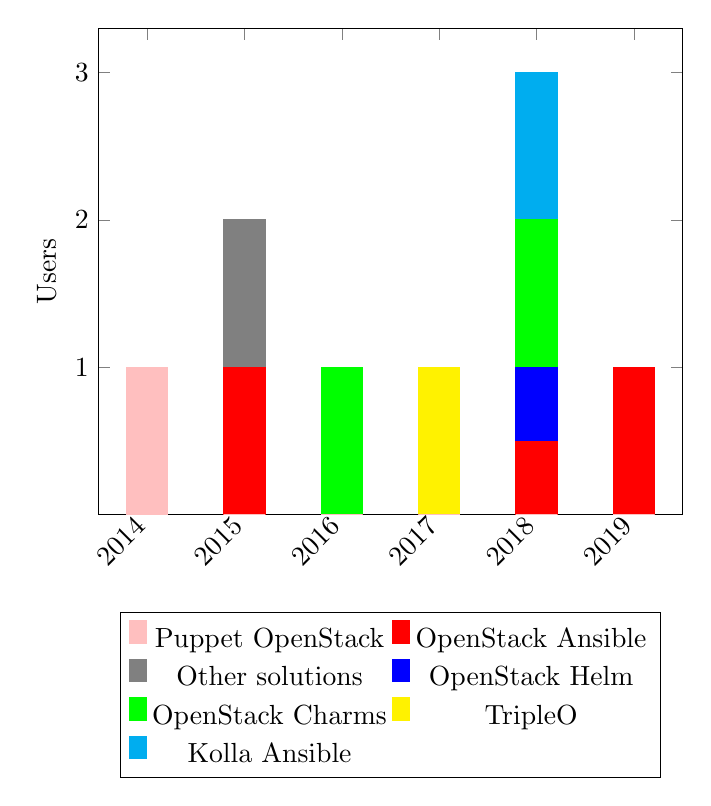
\begin{tikzpicture}
\begin{axis}[
    ybar stacked,
	bar width=15pt,
    ymin=0,
    ytick={1,2,3},
    legend style={
      cells={align=left},
      at={(0.5,-0.20)},
      anchor=north,legend columns=2
    },
    ylabel={Users},
    symbolic x coords={
      2014,
      2015,
      2016,
      2017,
      2018,
      2019},
    xtick=data,
    x tick label style={rotate=45,anchor=east},
    ]
% Puppet-OS
\addplot+[ybar,pink] plot coordinates {
  (2014,1)
  (2015,0)
  (2016,0)
  (2017,0)
  (2018,0)
  (2019,0)
};
% OS-Ansible
\addplot+[ybar,red] plot coordinates {
  (2014,0)
  (2015,1)
  (2016,0)
  (2017,0)
  (2018,.5)
  (2019,1)
};
% Other solutions
\addplot+[ybar,gray] plot coordinates {
  (2014,0)
  (2015,1)
  (2016,0)
  (2017,0)
  (2018,0)
  (2019,0)
};
% OS-Helm
\addplot+[ybar,blue] plot coordinates {
  (2014,0)
  (2015,0)
  (2016,0)
  (2017,0)
  (2018,.5)
  (2019,0)
};
% OS-Charms
\addplot+[ybar,green] plot coordinates {
  (2014,0)
  (2015,0)
  (2016,1)
  (2017,0)
  (2018,1)
  (2019,0)
};
% TripleO
\addplot+[ybar,yellow] plot coordinates {
  (2014,0)
  (2015,0)
  (2016,0)
  (2017,1)
  (2018,0)
  (2019,0)
};
% Kolla-Ansible
\addplot+[ybar,cyan] plot coordinates {
  (2014,0)
  (2015,0)
  (2016,0)
  (2017,0)
  (2018,1)
  (2019,0)
};
\legend{
  \strut Puppet OpenStack,
  \strut OpenStack Ansible,
  \strut Other solutions,
  \strut OpenStack Helm,
  \strut OpenStack Charms,
  \strut TripleO,
  \strut Kolla Ansible
}
\end{axis}
\end{tikzpicture}
\caption{Users of different methods as a distribution of adaptation year}
\label{fig:used-methods}
\end{figure}

\begin{figure}[t]
\centering
\resizebox{!}{5cm}{
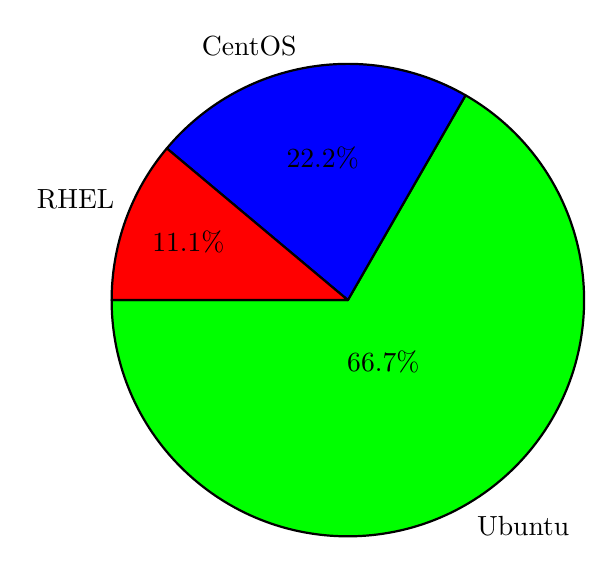
\begin{tikzpicture}
  \pie [rotate=180, color={green,blue,red}]
  {66.7/Ubuntu,
   22.2/CentOS,
   11.1/RHEL}
\end{tikzpicture}
}
\caption{Linux distributions used in target hosts}
\label{fig:used-distros}
\end{figure}

Questionnaire was sent to people from thesis work group contact network.
Altogether nine answers were received. Amount of answers was small due to
questionnare being sent to a relatvely small contact network and due to
aswering to it being voluntary. While providing small dataset, these facts make
the answer data more reliable on other aspects. It would be possible to repeat
the questionnaire to a larger respondent group and reflect those results to the
ones from the contact network. However in this thesis any comparisons from the
results will be done against OpenStack user surveys.

Most of the respondents worked in academic organizations. Countries where the
respondents were located were Denmark, Greece, Hungary, Norway, Sweden,
Switzerland, Finland and the Netherlands. According to OpenStack user surveys,
Europe has the third biggest user base of OpenStack, after Asia and North
America. Whether this affects the usefulness of automation form the
administrator's point of view is doubted.

All of the respondents were fairly experienced system administrators; more than
half had over ten years of professional IT working experience, with almost
half having twenty or more years of working experience. The experience of the
respondents provides some credibility. Earliest year for adapting a method was
2014. At highest the time of using the method has been a little over half of
the professional career of the respondent, more likely less than half of the
professional career. This would suggest that the respondent is unlikely to be
biased.

Almost all of the repondents considered system administrator as their role, on
third selecting product owner, and one project manager and software developer.
This was to be expected, but it was also insightful to see that so many of the
respondents also have responsibilities as product owner. This role may provide
them with more authority over decisions regarding selected tools.

Figure \ref{fig:used-methods} displays number of users for deployment methods
per year of adaptation. OpenStack-Ansible is the most used deployment method
with three users, one of which uses it in combination with OpenStack-Helm.
OpenStack-Charms is the second most used method with two users. Year of
adaptation does not indicate any specific trends with these two methods.

For other deployment methods, there is some correlation with the trends in the
community. Puppet-OpenStack, which is an early method for OpenStack deployment,
was adapted early, while container based methods, Kolla Ansible and OpenStack
Helm have been adapted more recently.

Majority of the respondents have not used other deployment methods for
production environments. While they possibly have used other methods for other
use purposes, such as proofs-of-concept, this indicates that the deployment
method chosen is not changed during operation.

Linux distributions used for target hosts are shown on Figure
\ref{fig:used-distros}. Ubuntu which has been the most widely used host
operating system according to OpenStack community user surveys, is used by more
than half of the respondents to this questionnaire as well.

Figure \ref{fig:other-software-configurations} displays correlations of the
used method to other software configurations. Only a minority does not or
cannot use the underlying automation tool for other software configurations.
This result suggests that automated deployment of OpenStack does not differ
crucially from other system deployments. Almost half of the respondents were
introduced to the automation tool by using it with OpenStack, but have since
started to use it for other software configurations.

\begin{figure}[t]
\centering
\resizebox{!}{5cm}{
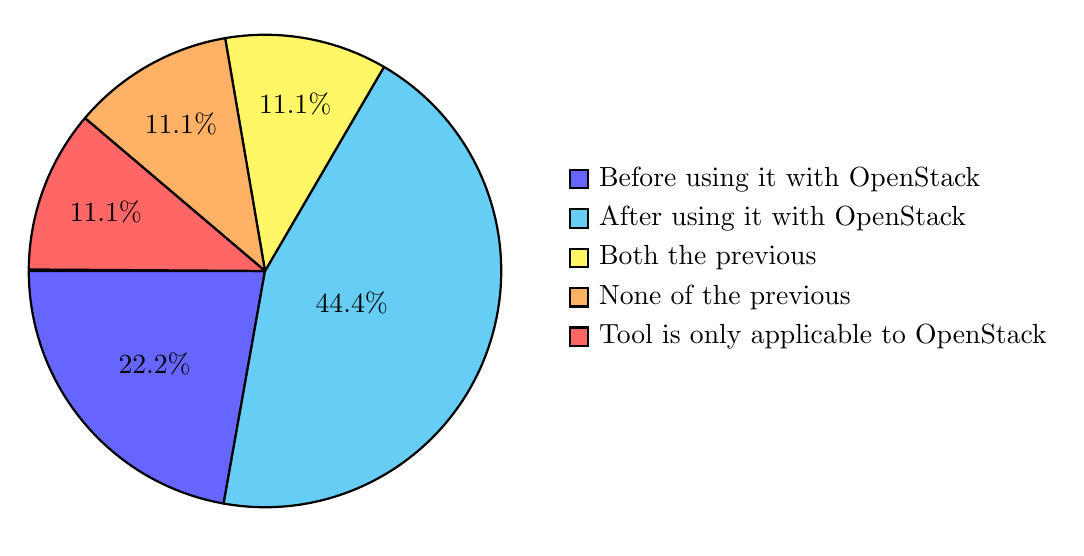
\begin{tikzpicture}
  \pie [text=legend, rotate=180] {
   22.2/Before using it with OpenStack,
   44.4/After using it with OpenStack,
   11.1/Both the previous,
   11.1/None of the previous,
   11.1/Tool is only applicable to OpenStack
  }
\end{tikzpicture}
}
\caption{Use of tool with other software configurations}
\label{fig:other-software-configurations}
\end{figure}

\begin{figure}[t]
\centering
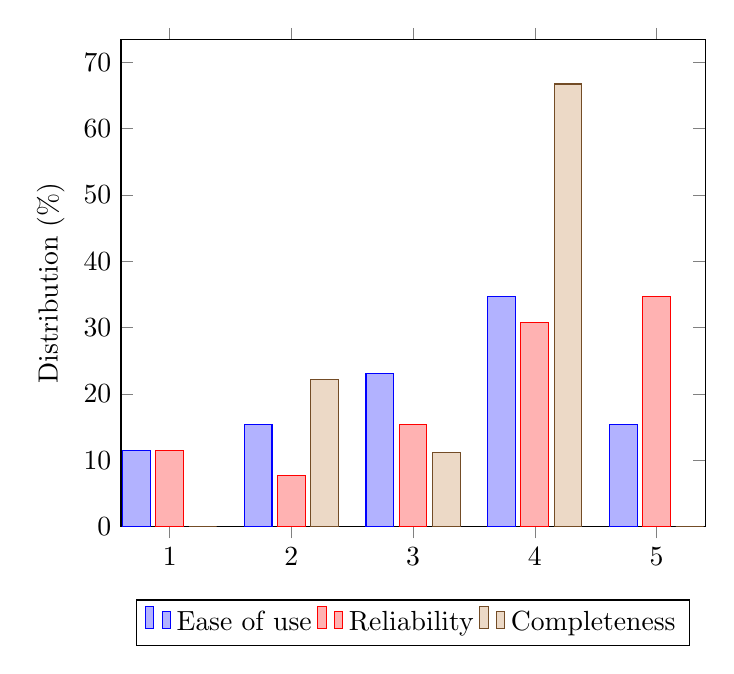
\begin{tikzpicture}
\begin{axis}[
    ybar,
    ymin=0,
    legend style={at={(0.5,-0.15)},
      anchor=north,legend columns=-1},
    ylabel={Distribution ($\%$)},
    symbolic x coords={1,2,3,4,5},
    xtick=data,
    ]
\addplot coordinates {(1,11.5) (2,15.4) (3,23.1) (4,34.6) (5,15.4)};
\addplot coordinates {(1,11.5) (2,7.7)  (3,15.4) (4,30.8) (5,34.6)};
\addplot coordinates {(1,0)    (2,22.2) (3,11.1) (4,66.7) (5,0)};
\legend{Ease of use,Reliability,Completeness}
\end{axis}
\end{tikzpicture}
\caption{Grading of deployment method}
\label{fig:method-grading}
\end{figure}

Results from grading the deployment methods are displayed on Figure
\ref{fig:method-grading}. Grade distributions for ease of use and reliability
are averages of distributions of questions 1-3 and 4-6 on Figure
\ref{fig:questionnaire-grading} correspondingly.

Ease of use is graded slightly above medium in average. Overall the
distribution is somewhat even showing no obvious trends. Correlation between
previous experience with the tool and professional experience in overall cannot
be analysed based on this testing due to the small data gathered. Previous
experience with software automation might make any deployment methods feel easy
which could affect this grading as well.

Reliability of the used automation tools is graded well, with highest frequency
grades being five and four. This is an important result as it points out that
reliability is one of the benefits of the use of automation.

Grading of completeness has more variance than the two other graded features.
One technical reason for this can be the fact that completeness had only one
graded scale, while distributions of usability and reliability are averaged
over three scales for different lifecycle operations. Regardless, the fact that
there were no highest or lowest grades given for completeness is unique for
this feature. Additionally, medium grade was the least frequent of given
grades, making the grade distribution of completeness different from other
features as well. Most frequent grading for completeness with biggest
difference from the next most frequent grade is four, providing a generally
positive evaluation.

Last optional question about any comments about the use of automation received
a few responses. One of the reponses pointed out how vendors can affect the
selection of tools, especially for smaller organizations; not relying on big
vendors like RedHat or Canonical for small organizations could even provide a
strategic risk. Another free text commented how easy adaptation of the tool is
important, but that the method should be customizable for later development.

\section{Hypothesis}

Results from the questionnaire provide some insight to answer research question
three in Figure \ref{fig:rqs} regarding the benefits of automated deployment
methods. While a larger scale questionnaire might represent the community with
more detail and provide data for more fine-grained analysis, some trends can be
seen from the received answers.

Even with a small set of respondents there are many different deployment
methods in use. Since the questionnaire focuses on the use of automated
solutions, it cannot be used for comparison with the use of manual deployments.
However the fact that such a wide variety of different methods are being used
suggests that there is no de facto solution for automating OpenStack
deployment.

The trends in the adaptation of different methods correlates to trends in the
OpenStack community. This is to be expected as the nature of OpenStack is
community-driven development. On top of that it is typical the the adapted
methods take influence from regional and organizational factors.

The fact that only a minority of respondents have not used the same automation
tool for other software configurations indicates that usefulness of software
configuration management often goes beyond deployment of a single software,
such as OpenStack. A big part of the respondents started using the tool after
being introduced to it by deploying OpenStack.

For the most part, the use of current automation methods is graded well in
terms of usability. Even though easiness did not get the highest grading for
the most, it got an overall positive grading. While usability is not generally
a priority on a tool used by professionals, many of the commercial software
products invest in it as well. For instance Puppet Enterprice provides a
browser based user interface, as does OpenStack Horizon.

Reliability is the most commonly seen benefit of the deployment methods
according to gradings in this questionnaire. While gradings of reliablity have
some variance, it distributes strongly towards positive grades with the highest
grade being the most frequent.

Used methods are graded well in terms of completeness, however it distributes
more unevenly than other features. This might indicate that there are some
varying opinions regarding how suitable different methods are for the current
needs of the deployment. It is a fact that automated deployment methods cannot
reach a higher level of configurability than manual configurations. However
the relatively positive grading in terms of completeness suggests that for many
users, the level of configurability with the used automation tool is sufficient
for the current needs.

In summary, conducted questionnaire suggests that mainly system administrators
benefit from the development of automated deployment methods. Use of automation
provides reliability for administrative tasks, while being easy to use and
sufficient for requirements.

\chapter{Evaluation} \label{evaluation}

OpenStack-Ansible deployment method was tested in a virtualized environment.
Method was picked due to its popularity in the results of questionnaire shown
on Chapter \ref{questionnaire} and its low-level nature. Scope of evaluation is
to explore the tasks needed for automated deployment of an operational
production-grade OpenStack cloud.

Goal of the evaluation is to provide more insight to research questions shown
on Figure \ref{fig:rqs} from one deployment method's point of view. Instead of
relying merely on reference literature, and available documentation, deployment
provides experience on low-level aspects to support other sources. According to
OpenStack user survey 2018 \cite{openstack-user-survey-2018}, documentation of
OpenStack is seen as one of the areas requiring improvements while at the same
time it is seen as one of the most appreciated aspects of OpenStack.

Deployment was kept as simple as possible while also being technically
sufficient for a production-grade environment. OpenStack production
environments differ from development environments much the same than any in any
software applications: production logging is less verbose and software running
in production mode is more optimized by omitting unnecessary functionality.

Many OpenStack development environment deployments utilize only a single
machine. With performant and reliable cloud deployment, services will have to
be distributed among multiple target machines, and deployment host containing
secrets such as authorized SSH keys and internal service credentials, has to be
separated from runtime enviroments for security reasons. Having separate
machine for deployment assets, makes it possible to have network-level security
policies. For instance SSH access to hosts running OpenStack services can be
allowed from the deployment hosts only.

Since production architectures are designed based on specific needs, deployment
is kept as simple as possible, with the possibility of extending functionality
according to custom needs. Thus there are only few requirements of the cloud
functionality. Basically it should be possible to create virtual networks and
virtual machines.

\section{Setup}

\begin{figure}[!b]
\centering

\begin{tikzpicture}[scale=.5]

\node[server](deploy-host){};
\node[server, left of= deploy-host, xshift=-1cm](target-host){};

\node[rack switch, above of=deploy-host,yshift=1cm]
  (management-switch){};
\node[rack switch, left of=management-switch, xshift=-1cm](tunnel-switch){};
\node[rack switch, left of=tunnel-switch, xshift=-1cm](storage-switch){};

\node[yshift=1cm, above of=management-switch,scale=0.2] (brouter) {\router{}};

\node[yshift=1cm,my cloud, minimum width=1.25cm, minimum height=1.55cm,
  above of=brouter,font=\large] (internet) {Internet};

% Label nodes
\node[below of = deploy-host,xshift=-1.5cm]{Deployment Host};
\node[below of = target-host,xshift=0.5cm]{Target Host};
\node[left of = management-switch,xshift=-2cm]{Management Network};
\node[above of = tunnel-switch,yshift=.5cm,xshift=.8cm,rotate=45]{Tunnel Network};
\node[above of = storage-switch,yshift=.5cm,xshift=.8cm,rotate=45]{Storage Network};
\node[left of = brouter,xshift=-1.5cm]{Gateway Router};

% Edges
\draw[thick,darkgray!10!gray] (deploy-host.north)--(management-switch);
\draw[thick,darkgray!10!gray] (target-host.north)--(management-switch);
\draw[thick,darkgray!10!gray] (target-host.north)--(tunnel-switch);
\draw[thick,darkgray!10!gray] (target-host.north)--(storage-switch);
\draw[thick,darkgray!10!gray] (brouter)--(management-switch);
\draw[thick,darkgray!10!gray] (internet)--(brouter);

\end{tikzpicture}

\caption{Test Setup Network Topology}
\label{fig:test-setup-network-topology}
\end{figure}

Setup used for test deployment simulates physical dataset topology depicted in
Figure \ref{fig:test-setup-network-topology}. Topology is based on deployment
guide of OpenStack-Ansible \cite{openstack-ansible}. By using virtual local
area networks, three separate physical switches as shown on the diagram would
not be needed, but instead a topology such as FatTree or Clos could be used in
a data center. Separate physical network devices do however ensure that
congestion in one network does not propagate to the other. It is also
recommended to use multiple physical network interfaces connected to separate
switches and bond them into the same bridge for redundancy.

In the simplest multi-node deployment setup, two hosts are used.
\textit{Deployment host} includes all of the assets needed for deployment,
including OpenStack-Ansible repository, Ansible roles used in deployment,
installation of Ansible, deployment configuration files, and secrets.
\textit{Target host} includes all of the OpenStack services and necessary
infrastructure services. When scaling deployment horizontally, instead of
having a single target host for all of the deployed software, setup could have
distinct hosts dedicated to compute services, storage services, and
infrastructure services.

\textit{Management network} is the only network routed to the Internet. It is
mainly used for management access to target host, and for egress internet
traffic. All of the hosts used in deployment will have to be connected to this
network. \textit{Tunnel network} is used for guest network traffic. Compute and
network nodes will have to be connected to it. \textit{Storage network} is used
for network volume traffic. Volume nodes are connected to it.

OpenStack cloud environment, called cPouta, provided by CSC Center for Science
Ltd. was used for virtualized test setup. While using a cloud service provides
benefits such as automated resource provisioning and configuration, it also
adds room for error. There is more components to troubleshoot when experiencing
issues. There may also be known issues in the cloud service that affect tasks
executed during evaluation. The same applies to any used software, including
operating systems. The benefits of using a cloud platform include fast and
automated infrastructure provisioning which makes testing more easily
repeatable.

Using virtualized environment as an infrastructure for testing differs from
physical data center in some aspects. Even though hypervisors can be run within
virtual machines and overlay networks can be constructed on top of existing
overlay networks, there are some details that have to taken into consideration
when deploying a cloud inside a cloud.

Since infrastructure provisioning is outside of the scope of OpenStack-Ansible,
host machines and virtual networks were provisioned with custom Heat stack
templates. Infrastructure provisioning from OpenStack cloud is conceptually
similiar to how TripleO uses undercloud or how Juju uses cloud providers.

Test environment was provisioned by using Heat orchestration tool. Heat
provisions servers for hosts and networks used in deployment. Additionally some
basic configurations were applied with cloud-init. Host configurations executed
with Heat make prerequisite system preparations shown on Figure
\ref{fig:osa-requirements}. Nameserver specified on the target host
\textit{resolv.conf} file had to be changed in order to provide functioning dns
resolution.

\begin{figure}[!b]
\centering
\begin{enumerate}
  \itemsep0em
  \item External network bridges are configured for nodes.
  \item SSH keys used in deployment are injected to target machines.
\end{enumerate}
\caption{Minimal prerequisites for OpenStack-Ansible multi-node deployment}
\label{fig:osa-requirements}
\end{figure}

Assumption with OpenStack-Ansible is that the subnets belong to separate VLANS.
With the test setup running in OpenStack, VXLAN segregation was used instead.
Difference with this approach is that, additional VLAN tagging is not employed
on guest hosts, but instead network interfaces are created by OpenStack
Neutron, and they are bridged without additional package tagging.

Ubuntu Bionic (18.04) was used for host machines. Since from release 17, Ubuntu
uses Netplan \cite{netplan} as the default network interface renderer. In order
to use legacy NetworkD service without additional setup programs, Netplan is
disabled and masked. Network bridges are then defined with NetworkD
configuration files.

\section{Deployment}

Once deployment host is prepared, OpenStack-Ansible repository includes shell
script for bootstrapping OpenStack Ansible deployment. Script installs Ansible
and the roles used in deployment. It hooks configuration files to be used in
OpenStack Ansible execution.

Once OpenStack Ansible is prepared, configuration files have to be installed on
the deployment server, which was done with a custom Ansible playbook.
OpenStack-Ansible uses three configuration files for describing the deployment.

\textit{openstack\_user\_config.yml} file describes which hosts are used for
particular services, and IP addressing. It maps different node types to
hostnames or IP addresses. Same IP can be used for multiple different node
types, and when OpenStack is deployed to a single host, all of the node groups
point to the same IP.

CIDRs for each of the configured networks are listed in
\textit{openstack\_user\_config.yml} file. Container network interfaces are
defined as well. Type of the mechanism used for plugging container interfaces
to appropriate network bridges can be specified in configuration. Virtual
ethernet pairs were used in the test deployment as it is the most common
mechanism according to OpenStack-Ansible documentation
\cite{openstack-ansible}.

Most of the configurations specified in \textit{openstack\_user\_config.yml}
file do not need to be specified with some of the other deployment methods such
as Kolla Ansible or OpenStack Charms. More high-level deployment methods can
provide a default configuration for network bridges and container interfaces.
These bridges could also be configured automatically for a proof-of-concept
installation with OpenStack-Ansible. Reason for low-level network configuration
is likely the fact that OpenStack-Ansible is used for data center deployments
with varying topologies. While providing more configurability, this method has
potential for error due to environment setup not matching the configuration
specified for OpenStack-Ansible.

\textit{user\_variables.yml} defines parameters used by Ansible roles in
deployment. Many of the specified parameters describe configuration parameters
used for the installed programs, but some specify installation features.

In order to get the deployment functioning, HTTPS protocol had to be specified
for public, internal, and administrative api endpoints, and TLS verification
had to be set off. Without these specifications some of the verification tasks
failed due to Ansible trying to use HTTP requests for HTTPS endpoints, or due
to warnings about untrusted self-signed TLS certifiates.

Default installation method is to used source code and install programs with
pip into virtual enviroments. While this method takes longer than using
prepared distribution packages it is the most reliable method for test
deployments, since it guarantees that appropriate versions are being used for
OpenStack services. New OpenStack releases are not always published to public
repositories for package managers such as apt or yum. For long term operations
it would be possible to create custom distribution packages for new OpenStack
releases.

While providing a minimal required configuration for a successful deployment,
in a production level deployment TLS verification would not have to be turned
off, since the deployer would likely provide certificates signed by a trusted
authority. There would likely be other configuration variables that would be
specified according to custom needs. However a simple deployment can be run
successfully with five specified configuration parameters in
\textit{user\_variables.yml} file.

Third configuration file, \textit{user\_secrets.yml} contains secrets used in
deployment, including credentials to various services used by administrators
and other deployed service users. OpenStack-Ansible repository includes a
Python script for generating random secrets. While having all of the deployment
secrets in a single file makes it easier to leak all of the passwords at the
same time, it has benefits as well. For deployer it provides easy access to all
of the deployed services without having to separately read a distinct file for
service to be accessed. Proper secret management is not part of the scope of
OpenStack-Ansible, and other solutions for it can be used as needed.

In case some of the secrets would leak, generating new ones with the script
would be fast. However installation playbook is not idempotent and thus using
it as a methods for disaster recovery would require the entire OpenStack to be
re-installed. Depending on how this is done it could have a big impact on the
service operation.

After preparation, OpenStack can be installed according to configurations by
running a single Ansible playbook. Installation consists of three phases and
in test setup it took approximately two hours when installing from source code.
First Ansible prepares target hosts. During this phase LXC containers for each
of the services are initialized and plugged into networks. During the second
phase the infrastructure services required by OpenStack services are installed
and configured. Finally OpenStack services themselves are installed according
to configuration specifications.

\section{Verification}

As with any software, verification of an operational OpenStack deployment
depends on the expected functionality. With any requirements however, there are
some indications of a failed deployment, such as SystemD services in failed
state or network connectivity issues. After running Ansible playbooks
successfully, these features were checked with operating system functionality
and network diagnostic tools. Many of the basic issues such as problems with
connectivity, will likely result in failed playbook execution.

Approaches to verifying software configurations can be highly analytical, and
based on static checks. Rehearsal \cite{rehearsal} is a software developed for
verifying system configurations applied with puppet. While similiar tools can
be created for other software configuration management tools, this paper
focuses on core functionality which is simple enough to verify manually.

OpenStack-Ansible includes tasks for both setting up some basic resources such
as provider networks and machine images, as well as verifying functional cloud
by using automated tests. These features can be enables with configuration
parameters. These tasks were not used in evaluation in order to focus on the
core deployment functionality. In order to provide transparent testing of the
deployment, running the basic verification operations manually was seen
sufficient. Once the deployment is confirmed functional these tasks could
be used for further cloud deployments.

The initial deployment is difficult to keep as small as adding a single service
at a time. It entails a lot of tasks that depend on one another. For this
reason it is kept as simple as possible while enabling expansion as potential
future work.

For verifying operational deployment, tasks shown on Figure
\ref{fig:verify-tasks} were executed. Tasks verify the functionality of most
essential OpenStack services, Keystone, Glance, Neutron, and Nova. More
services can be added, once the basic services are confirmed operational.

CirrOS image used for virtual machine testing is a machine image commonly used
for verifying OpenStack deployment. Its raw image file was downloaded from the
official source and provided for Glance API in image creation request.

Once machine image was uploaded successfully, tenant network was created for
virtual machines. With tenant network created, host flavor for virtual machines
had to be created. With an image, network and a flavor guest hosts could be
created to verify that Nova API works properly. When plugging guest hosts to
the same tenant network, connectivity can be verified by using tenant network
private ip addresses. For ICMP network diagnostics ingress firewall rules have
to be set up accordingly.

While functionality verified for the test setup contains only a subset of
necessary features of an operational OpenStack deployment, it was sufficent to
confirm that the deployment matched the specified configuration. Some of the
deployed features were not verified as they were not seen necessary for
providing answers to research questions. Verification performed during the
evaluation is sufficient to bring out features offered by OpenStack-Ansible
deployment method as well as its benefits and tradeoffs. Any further
enhancements to the deploymet could be left as future work.

\begin{figure}[t]
\centering
\begin{enumerate}
  \itemsep0em
  \item Upload CirrOS image to Glance.
  \item Create private Neutron network and subnet.
  \item Enable ICMP ingress security group rule in default security group.
  \item Create test flavor for virtual machines.
  \item Create two Nova virtual servers in private network using CirrOS image.
  \item Open console session with virsh to one of the created Nova servers.
  \item Confirm network access between the two deployed servers by pinging one
        from the other.
\end{enumerate}
\caption{Verification tasks for deployment}
\label{fig:verify-tasks}
\end{figure}

\section{Hypothesis}

Designing and deploying a testbed for OpenStack-Ansible provided clarified how
automated deployments for OpenStack are prepared and executed. Not many manual
administrative tasks were required during deployment. However due to Ansible's
verbose logging and descriptive task naming, it was easy to see which tasks
were executed during deployment. Tasks describe what configuration items are
involved in deployment, and what kind of configurations are applied.

To answer research question RQ1 in Figure \ref{fig:rqs}, one of the key factor
affecting the design of OpenStack-Ansible is the ability to provide automated
deployment of OpenStack on top of a pre-existing server infrastructure. This
choice provides configurability at the cost of having to carry the
responsibility of low-level setup of the infrastructure. In comparison to some
of the other deployment methods, OpenStack-Ansible architecture has to be
designed in detail before the deployment. The deployment configuration has
correspond to the existing infrastructure. This design is fundamental to
OpenStack-Ansible which provides a batteries-included deployment method, as
stated in its manifest \cite{openstack-ansible}.

Getting started with using OpenStack-Ansible for a multi-node deployment was
not as easy as using a development environment setup, such as Packstack.
Getting the deployment working required multiple trials and some
troubleshooting. Installing OpenStack services manually might be more easy in
the beginning. However with automation tools once the issues were resolved the
deployment could be repeated easily. This applied also to infrastructure
provisioning with Heat. Even though it was not tested, automated deployment is
likely to scale better than manual installation.

Ideally when a change in the configuration of the production environment would
have to be made, the configuration could be properly tested in a staging
environment and the be run in production environment avoiding operational
errors. This approach requires a testbed that is structurally similiar to the
production environment. Since hosts can be accurately emulated by using
hypervisors, network setup used in evaluation was the most different from a
datacenter network, since VLAN provisioning was not available in the used
OpenStack platform.

Due to OpenStack deployment test setups never totally matching production
environments, there is always room to question the benefit of automated
deployment methods as experienced in a test. However based on the experiences
during evaluation, use of software automation shows a lot of potential for
deployment of OpenStack production environment. Reliability which was seen as
one of the strengths of automated deployment methods in questionnaire on
Chapter \ref{questionnaire} could be confirmed as it was to reproduce once
successfully executed deployment.

Features listed above benefit primarily system administrators, as they would be
the ones running the configurations manually otherwise. In case of issues, the
administrators would still have do the troubleshooting. If the deployment is
configured correctly, administrators do not have to worry about applying the
configuration to the targeted system. While repeating the same configuration
tasks creates a routine for the administrator, when updates are applied to the
system, some of the confiuration tasks may be new and require some prior
testing.

In addition to administrators benefiting from the development of automation
tools, developers benefit from it as well. Software developers have a tendency
to focus on application development and not environment setups. Due to Ansible
playbooks describing environment setup tasks concretely, they function as a
type of documentation. This could be seen during evaluation of OpenStack
Ansible when at one point a role was resulting in failure. The role's tasks
described in YAML format, provided detailed description of the task that was
run. Combining this description to the error log enabled the root issue to be
revealed and fixed. This process brought out some details of the overall
deployment.

The evaluation of OpenStack Ansible provided an introduction to automated
deployment of OpenStack. Not using an all-in-one deployment method but instead
configuring an optimized deployment required understanding of both OpenStack
services, underlying infrastructure services as well as networking concepts
related to both the test environment and LXC containers. Evaluation brought out
some details that were not found in any documentation. It is common in a large
software stack for some details to change constantly. Keeping documentation up
to date with these changes is difficult. For this reason it is often stated in
the documentation to consult the documentation of any software dependencies
directly instead.

OpenStack-Ansible provided very little features as a deployment method.
Following the design principle of Ansible, OpenStack-Ansible included no other
configuration items that deployment host, which had to be prepared by the
deployer. Most of the work during the evaluation was related the preparation of
the deployment and not the configuration of the actual deployment. This is
characteristic to OpenStack-Ansible. It is agnostic of the underlying
infrastructure and focuses on automating the configuration operations only.

Once deployment was configured properly, its execution succeeded without
exception. Reliability from administrator's point of view, which was one of the
key findings of questionnaire in Chapter \ref{questionnaire} could thus be
confirmed during this evaluation. Other benefits of configuration management
tool included easy execution. Configuration file sources made it easier to
learn how OpenStack is deployed.

\chapter{Summary}

This paper has presented contemporary methods for automating configuration
tasks for a cloud platform deployment. Different designs, as well as tools and
components included in deployment methods have been introduced. Other
differences between methods have been explored as well. Lastly, some of the
benefits of the development of automated tools have been presented and
reasoned.

Answers to research questions shown on Figure \ref{fig:rqs} are based on
reference publications, technical documentation, a small scale questionnaire,
as well as a deployment test conducted in a virtualized environment. There have
not been conflicting results gained from different sources although some of the
methods focus on different aspects of the research.

Topic of this paper is motivated by contemporary practices in IT infrastructure
management utilizing cloud computing and popularity of automating system
configuration tasks. These trends have emerged from years of providing
large scale internet-based services. Recent developments in virtualization
technologies have helped to automate different administrative tasks. At the
same time organizations adapting agile philosophies for IT service management
has created need to increase the level of automation in service management.

Cloud computing has provided scalable infrastructure for services provided over
the internet. Cloud platforms can provide infrastructure as a service for
external organizations or different departments in the same organization. Cloud
platforms are administered much the same way than other IT services. In order
to be profitable cloud platforms need to be large. Administrative tasks in
cloud datacenters can become time-consuming, difficult, and entail a lot of
operational risks.

OpenStack is a family of open-source software projects for running cloud
platform. It has been developed by various organizations and community
contributions. Currently OpenStack is the most commonly used software for
running private clouds. It is being used by big organizations in
telecommunication, retail, finance and scientific research. Systm
architecturally OpenStack bears close resemblance to other popular public cloud
platforms AWS, Azure and GCP.

Software configuration management has become a popular solution for
administering datacenters. It provides means to create configurations that are
applied to the system by a computer program. While there are technically no
limits to configurations that can be applied with automated tools, different
tools provide varying functionality. Automation tools have different software
architectures that affect how complex configuration tasks are structured.

OpenStack community has created various official deployment methods that
utilize software configuration management tools. Deployment methods follow best
practices of the underlying automation tools and focus on configuring OpenStack
services to available server infrastructure. Some deployment methods include
infrastructure provisioning while others are run against pre-existing server
infrastructure. Design of different automated deployment methods is driven by
their use purposes. Methods may focus on easy adaptation, extendability,
configurability or operability with varying emphasis.

Some of the deployment methods only include assets for an initial deployment of
OpenStack. Further operation and maintenance would then have to be provided
with custom solutions or by using other tools available. Other deployment
methods include functionality for scaling, updating, or health monitoring the
deployment. The latter type of deployment methods usually contains more
configuration items, whose operation has to be assured during cloud operations.
The former type does often not include any additional software dependencies
than tool used for the deployment itself.

There are parties that may benefit from the use of automation tools indirectly.
In case automation can be used for providing high quality service in an
affordable fashion, both the service providers and end users benefit from it.
While hhis benefit may even seem obvious it is difficult to prove, since the
actual measurements on savings can be complex and a subject to non-disclosure.

Since automated tools are primarily used by system administrators, they are the
primary beneficiaries from the development of the tools. Results from
questionnaire presented in Chapter \ref{questionnaire} suggest that system
administrators benefit from reliability when using automated software
configuration tools. Reliability was also noticable in evaluation shown on
Chapter \ref{evaluation} as succesful execution was easily repeatable.

At the moment it would seem that the use of automated solutions for system
administration will keep on gaining popularity. Since use of automation in
general is increasing and being applied in areas such as decision making, using
it to be able to automate system administration tasks is not totally
unexpected. In addition to providing reliability for repeating tasks, it may
even create new possibilities for management of large scale IT infrastructures.

There are no obvious solutions or de facto software for automating
infrastructure management, although some methods are more popular than others.
Even though some methods will inevitably become deprecated at some point, the
need for automation for infrastructure management has a number of reasons to
stay relevant.


%%%%%%%%%%%%%%%%%%%%%%%%%%%%%%%%%%%%%%%%%%%%%%%%%%%%%%%%%
\cleardoublepage                          %fixes the position of bibliography in bookmarks
\phantomsection
\addcontentsline{toc}{chapter}{\bibname}  % This lines adds the bibliography to the ToC
\printbibliography

%%%%%%%%%%%%%%%%%%%%%%%%%%%%%%%%%%%%%%%%%%%%%%%%%%%%%%%%%
%\backmatter
%\begin{appendices}

%\end{appendices}
%%%%%%%%%%%%%%%%%%%%%%%%%%%%%%%%%%%%%%%%%%%%%%%%%%%%%%%%%

\end{document}
